% ============================================================
%  Span2Type -- Master's Thesis Defense Slides
%  Compile with:  xelatex defense-slides.tex  (twice for refs)
%  or:  latexmk -xelatex defense-slides.tex
% ============================================================
\documentclass[aspectratio=169,10pt]{beamer}

% ---- packages ------------------------------------------------
\usepackage{fontspec}
\usepackage{amsmath,amsfonts,amssymb}
\usepackage{booktabs}
\usepackage{multirow}
\usepackage{colortbl}
\usepackage{graphicx}
\usepackage{xcolor}
\usepackage{array}
\usepackage{tabularx}
% pifont conflicts with fontspec/XeLaTeX; use amssymb symbols instead
\usepackage{tikz}
\usetikzlibrary{shapes.geometric,arrows.meta,positioning,
                fit,backgrounds,decorations.pathreplacing,calc}
\usepackage{pgfplots}
\pgfplotsset{
  compat=1.18,
  tick label style={font=\normalfont\small},
  label style={font=\normalfont\small},
  legend style={font=\normalfont\tiny},
  title style={font=\normalfont\small}
}

% ---- fonts (XeLaTeX) ----------------------------------------
\setmainfont{TeX Gyre Termes}
\setsansfont{TeX Gyre Heros}[Scale=MatchLowercase]
\setmonofont{TeX Gyre Cursor}[Scale=MatchLowercase]

% ---- colors -------------------------------------------------
\definecolor{navyblue}{RGB}{0,51,102}
\definecolor{gold}{RGB}{204,160,0}
\definecolor{lightblue}{RGB}{220,232,245}
\definecolor{dkgreen}{RGB}{0,110,55}
\definecolor{dkred}{RGB}{160,20,20}
\definecolor{greycell}{RGB}{240,240,240}

% ---- beamer theme -------------------------------------------
\usetheme{Madrid}

\setbeamercolor{palette primary}{bg=navyblue,fg=white}
\setbeamercolor{palette secondary}{bg=navyblue!85!black,fg=white}
\setbeamercolor{palette tertiary}{bg=navyblue!70!black,fg=white}
\setbeamercolor{palette quaternary}{bg=navyblue,fg=white}
\setbeamercolor{frametitle}{bg=navyblue,fg=white}
\setbeamercolor{title}{bg=navyblue,fg=white}
\setbeamercolor{subtitle}{fg=gold}
\setbeamercolor{structure}{fg=navyblue}
\setbeamercolor{itemize item}{fg=navyblue}
\setbeamercolor{itemize subitem}{fg=gold!80!black}
\setbeamercolor{enumerate item}{fg=navyblue}
\setbeamercolor{block title}{bg=navyblue,fg=white}
\setbeamercolor{block body}{bg=lightblue,fg=black}
\setbeamercolor{block title alerted}{bg=dkred,fg=white}
\setbeamercolor{block body alerted}{bg=dkred!10,fg=black}
\setbeamercolor{block title example}{bg=dkgreen,fg=white}
\setbeamercolor{block body example}{bg=dkgreen!10,fg=black}
\setbeamercolor{alerted text}{fg=dkred}

\setbeamerfont{title}{size=\large,series=\bfseries}
\setbeamerfont{subtitle}{size=\normalsize,series=\mdseries}
\setbeamerfont{frametitle}{size=\normalsize,series=\bfseries}
\setbeamerfont{block title}{size=\small,series=\bfseries}

\setbeamertemplate{navigation symbols}{}
\setbeamertemplate{itemize item}[circle]
\setbeamertemplate{itemize subitem}[triangle]

% Custom footline: left = current section, center = short title, right = page n/N
\setbeamertemplate{footline}{%
  \leavevmode%
  \hbox{%
    \begin{beamercolorbox}[wd=0.3\paperwidth,ht=2.25ex,dp=1ex,
                           left,leftskip=1em]{palette secondary}%
      \usebeamerfont{author in head/foot}\insertsection
    \end{beamercolorbox}%
    \begin{beamercolorbox}[wd=0.4\paperwidth,ht=2.25ex,dp=1ex,
                           center]{palette primary}%
      \usebeamerfont{title in head/foot}\insertshorttitle
    \end{beamercolorbox}%
    \begin{beamercolorbox}[wd=0.3\paperwidth,ht=2.25ex,dp=1ex,
                           right,rightskip=1em]{palette secondary}%
      \usebeamerfont{date in head/foot}%
      \insertframenumber\,/\,\inserttotalframenumber
    \end{beamercolorbox}%
  }%
}

% ---- helper commands ----------------------------------------
\newcommand{\hl}[1]{\textcolor{gold!80!black}{\textbf{#1}}}
\newcommand{\hb}[1]{\textcolor{navyblue}{\textbf{#1}}}
\newcommand{\hg}[1]{\textcolor{dkgreen}{\textbf{#1}}}
\newcommand{\hr}[1]{\textcolor{dkred}{\textbf{#1}}}
\newcommand{\cmark}{\textcolor{dkgreen}{$\checkmark$}}
\newcommand{\xmark}{\textcolor{dkred}{$\times$}}
\newcommand{\pmark}{\textcolor{gold!80!black}{$\diamond$}}

% placeholder box for missing figures
\newcommand{\figph}[2][7.5cm]{%
  \begin{center}
    \begin{tikzpicture}
      \node[draw=navyblue!40,fill=lightblue!50,rounded corners=4pt,
            minimum width=#1,minimum height=3.2cm,
            font=\small\itshape,text width=#1-0.6cm,align=center]{#2};
    \end{tikzpicture}
  \end{center}}

% section divider slide
\newcommand{\sectionslide}[2]{%
  \begin{frame}[plain]
    \begin{tikzpicture}[remember picture,overlay]
      \fill[navyblue] (current page.north west) rectangle (current page.south east);
      \node[font=\Huge\bfseries,white,align=center] at (current page.center) {#1};
      \node[font=\large,gold,align=center,yshift=-1.2cm] at (current page.center) {#2};
    \end{tikzpicture}
  \end{frame}}

% ---- metadata -----------------------------------------------
\title[Span2Type: Open World NER]{Span2Type: Open World Named Entity Recognition with Automatic Entity Naming}
\subtitle{Master's Thesis Defense}
\author[KhoaNguyen]{%
  \textbf{Nguyen Anh Khoa} \\[0.2em]
  {\small Student ID: M1261026} \\
  {\small Advisor: Supervisor: Prof.\ [Hsien-Tsung CHANG 張賢宗]}%
}
\institute[AI Dept -- CGU]{%
  Graduate Institute of Artificial Intelligence \\
  Chang Gung University, Taiwan%
}
\date{April 2026}

% =============================================================
\begin{document}
% =============================================================

% ------------------------------------------------------------------
% SLIDE 1 — TITLE
% ------------------------------------------------------------------
\begin{frame}[plain]
  \begin{tikzpicture}[remember picture,overlay]
    \fill[navyblue] (current page.north west) rectangle (current page.south east);
    % Place CGU on top-left and AI Dept on top-right.
    \node[anchor=north west,inner sep=0pt,xshift=0.9cm,yshift=-0.45cm]
      at (current page.north west) {
\includegraphics[height=0.95cm]{cgu logo2.png}};
    \node[anchor=north east,inner sep=0pt,xshift=-0.9cm,yshift=-0.45cm]
      at (current page.north east) {
\includegraphics[height=0.95cm]{aidept logo.png}};
    \node[anchor=north,yshift=-1.45cm,font=\Large\bfseries,white,align=center,text width=0.88\paperwidth]
      at (current page.north)
      {Span2Type: Open World Named Entity Recognition\\with Automatic Entity Naming};
    \node[font=\small,gold,align=center,yshift=-0.75cm]
      at (current page.center) {Master's Thesis Defense};
    \node[font=\small,white!80,align=center,yshift=-1.85cm]
      at (current page.center){%
        Nguyen Anh Khoa \quad|\quad Student ID: M1261026 \\[3pt]
        Advisor: Supervisor: Prof.\ [Hsien-Tsung CHANG 張賢宗] \\[5pt]
        Graduate Institute of Artificial Intelligence\\
        Chang Gung University, Taiwan\\
        April 2026};
  \end{tikzpicture}
\end{frame}

% ------------------------------------------------------------------
% SLIDE 2 — OUTLINE
% ------------------------------------------------------------------
\begin{frame}{Outline}
  \begin{columns}[T]
    \begin{column}{0.5\textwidth}
      \tableofcontents[sections={1-4},hideallsubsections]
    \end{column}
    \begin{column}{0.5\textwidth}
      \tableofcontents[sections={5-7},hideallsubsections]
    \end{column}
  \end{columns}
  \vspace{0.5em}
  \begin{tikzpicture}
    \draw[navyblue!30,line width=0.4pt] (0,0) -- (12cm,0);
  \end{tikzpicture}
  \vspace{0.2em}
 
\end{frame}

% =============================================================
\section{Problem Statement}
% =============================================================

% ------------------------------------------------------------------
% SLIDE 3 — REAL-WORLD NER
% ------------------------------------------------------------------
\begin{frame}{Named Entity Recognition — The Benchmark vs.\ Reality Gap}
  \begin{columns}[T]
    \begin{column}{0.48\textwidth}
      \textbf{What NER does (closed benchmarks)}
      \begin{itemize}
        \item Locate entity spans in text
        \item Classify into \textit{fixed, predefined} types:\\
          \textsc{Person} · \textsc{Org} · \textsc{Location}
        \item BERT/RoBERTa: near-human F1 on CoNLL-2003
      \end{itemize}
      \vspace{0.4em}
      % \begin{alertblock}{The hidden assumption}
      %   Type inventory is \textbf{fixed} at training time.
      %   Labeled data must \textbf{exist} for every type.
      % \end{alertblock}
    \end{column}
    \begin{column}{0.5\textwidth}
      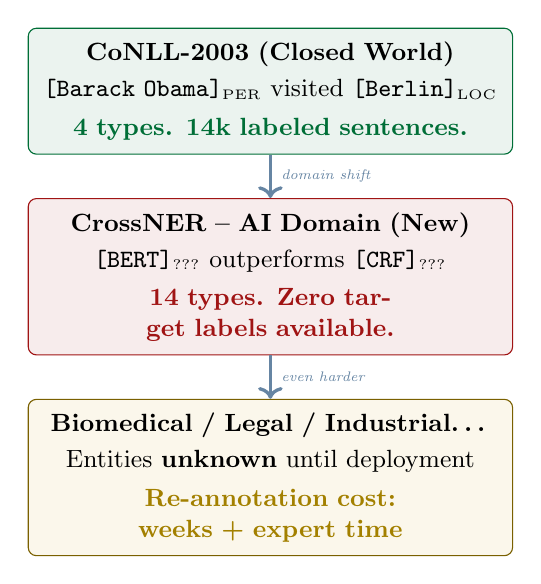
\begin{tikzpicture}[node distance=0.55cm,
          box/.style={draw,rounded corners=3pt,
                      text width=5.8cm,align=center,
                      inner sep=5pt,font=\small}]
        \node[box,draw=dkgreen,fill=dkgreen!8] (a) {
          \textbf{CoNLL-2003 (Closed World)}\\[2pt]
          \texttt{[Barack Obama]}\textsubscript{\tiny PER}
          visited \texttt{[Berlin]}\textsubscript{\tiny LOC}\\[3pt]
          \hg{4 types. 14k labeled sentences.}
        };
        \node[box,draw=dkred,fill=dkred!8,below=of a] (b) {
          \textbf{CrossNER -- AI Domain (New)}\\[2pt]
          \texttt{[BERT]}\textsubscript{\tiny ???}
          outperforms
          \texttt{[CRF]}\textsubscript{\tiny ???}\\[3pt]
          \hr{14 types. \textbf{Zero} target labels available.}
        };
        \node[box,draw=gold!60!black,fill=gold!8,below=of b] (c) {
          \textbf{Biomedical / Legal / Industrial…}\\[2pt]
          Entities \textbf{unknown} until deployment\\[3pt]
          \hl{Re-annotation cost: weeks + expert time}
        };
        \draw[->,very thick,navyblue!60] (a.south) -- (b.north)
          node[midway,right,font=\tiny\itshape]{domain shift};
        \draw[->,very thick,navyblue!60] (b.south) -- (c.north)
          node[midway,right,font=\tiny\itshape]{even harder};
      \end{tikzpicture}
    \end{column}
  \end{columns}
\end{frame}

% ------------------------------------------------------------------
% SLIDE 4 — THREE CHALLENGES
% ------------------------------------------------------------------
\begin{frame}{Three Concrete Deployment Challenges}
  \begin{columns}[T]
    \begin{column}{0.32\textwidth}
      \begin{block}{\#1 \ Domain Shift}
        BIO tagger trained on newswire\\fails on AI / bio / legal text.\\[4pt]
        Multi-token technical entities:\\
        \emph{support vector machine}\\
        \emph{recurrent neural network}\\[4pt]
        Single-view BIO misses boundaries.
      \end{block}
    \end{column}
    \begin{column}{0.32\textwidth}
      \begin{block}{\#2 \ Unknown Type Inventory}
        New domains have:\\
        $\bullet$ Finer-grained types\\
        $\bullet$ Entirely new categories\\
        $\bullet$ Evolving terminology\\[4pt]
        Supervised models cannot\\discover \emph{new} types.\\
        Need: automatic $k$ selection.
      \end{block}
    \end{column}
    \begin{column}{0.32\textwidth}
      \begin{block}{\#3 \ Interpretability Gap}
        Unsupervised clustering produces:\\[4pt]
        \quad \emph{Cluster 3}, \emph{Cluster 7}, \ldots\\[4pt]
        Anonymous IDs $\to$ expert must\\
        manually inspect \& label.\\[4pt]
        Defeats the purpose of\\unsupervised discovery.
      \end{block}
    \end{column}
  \end{columns}
  \vspace{0.5em}
  \begin{center}
    \small
    \begin{tabular}{lcccc}
      \toprule
      \textbf{Method} & \textbf{Ch.\,1 Span Detection} & \textbf{Ch.\,2 Auto-k Typing} & \textbf{Ch.\,3 Naming} \\
      \midrule
      Supervised NER   & \xmark & \xmark & \xmark \\
      Few-shot NER     & \pmark & \xmark & \xmark \\
      OWNER (baseline) & \pmark & \cmark & \xmark \\
      \textbf{Span2Type (ours)} & \cmark & \cmark & \cmark \\
      \bottomrule
    \end{tabular}
  \end{center}
\end{frame}

% =============================================================
\section{Background \& Related Work}
% =============================================================

% ------------------------------------------------------------------
% SLIDE 5 — NER LANDSCAPE
% ------------------------------------------------------------------
\begin{frame}{NER: From CRFs to Transformers}
  \begin{tikzpicture}[remember picture,overlay,
      dot/.style={circle,fill=navyblue,inner sep=2.5pt},
      ev/.style={font=\small,text width=3.5cm,align=center}]
    % Timeline arrow
    \draw[->,very thick,navyblue!40] (0.5,3) -- (14.5,3);
    \foreach \x/\yr in {1.5/2001,4.5/2016,7.5/2019,11/2022,13.5/2024}
      \node[dot] at (\x,3) {};
    \foreach \x/\yr in {1.5/2001,4.5/2016,7.5/2019,11/2022,13.5/2024}
      \node[font=\tiny,navyblue,below=3pt] at (\x,3) {\yr};
    % Labels
    \node[ev,above=0.5cm] at (1.5,3) {\small CRF\\(Lafferty '01)\\F1 \textasciitilde89\%};
    \node[ev,above=0.5cm] at (4.5,3) {\small BiLSTM-CRF\\(Ma '16)\\F1 \textasciitilde91\%};
    \node[ev,above=0.5cm] at (7.5,3) {\small BERT\\(Devlin '19)\\F1 \textasciitilde92.8\%};
    \node[ev,above=0.5cm] at (11,3)  {\small Few-shot\\cross-domain\\NER};
    \node[ev,above=0.5cm] at (13.5,3){\small Open-world\\NER\\OWNER '23};
  \end{tikzpicture}
  \vspace{2.8cm}
  \begin{columns}[T]
    \begin{column}{0.5\textwidth}
      \textbf{Common limitation across all eras:}
      \begin{itemize}
        \item Require predefined type inventory
        \item Need at least a few labeled examples per type
        \item Cannot discover \emph{new} entity categories
      \end{itemize}
    \end{column}
    \begin{column}{0.5\textwidth}
      \textbf{Open-world NER removes all constraints:}
      \begin{itemize}
        \item No predefined types
        \item No target-domain annotations
        \item Discovers types automatically via clustering
      \end{itemize}
    \end{column}
  \end{columns}
\end{frame}

% ------------------------------------------------------------------
% SLIDE 5b — SPAN DETECTION PRIOR WORK
% ------------------------------------------------------------------
\begin{frame}{Related Methods — Span Detection Approaches}
  \begin{columns}[T]
    \begin{column}{0.48\textwidth}
      \textbf{Sequence tagging (BIO):}
      \begin{itemize}\setlength{\itemsep}{1pt}
        \item Standard: BERT/DeBERTa + single BIO head
        \item \hr{Error propagation}: wrong B tag corrupts entire span
        \item Single boundary signal — easily confused cross-domain
      \end{itemize}
      \vspace{0.35em}
      \textbf{Span enumeration (PURE, Chen '21):}
      \begin{itemize}\setlength{\itemsep}{1pt}
        \item Enumerate all $\mathcal{O}(n^2)$ candidate spans explicitly
        \item No boundary cascading errors
        \item \hr{Weak cross-domain transfer} — F1 35.8 avg on CrossNER
      \end{itemize}
      \vspace{0.35em}
      \textbf{Prototype / coref-based detection:}
      \begin{itemize}\setlength{\itemsep}{1pt}
        \item \textbf{SpanProto}: prototype matching — F1 61.0 avg
        \item \textbf{WL-Coref}: coreference boundaries — F1 65.6 avg
        \item Still limited to a \emph{single} detection view
      \end{itemize}
    \end{column}
    \begin{column}{0.48\textwidth}
      \textbf{Multi-view ensemble (DTrans, Zheng '22):}
      \begin{itemize}\setlength{\itemsep}{1pt}
        \item Three complementary decoders trained jointly:\\
              \quad\textbf{BIO} + \textbf{Start-End (SE)} + \textbf{Tie-Break (TB)}
        \item Mean Teacher EMA enforces cross-view consistency
        \item Errors in one view cancelled by consensus of others
        \item \hg{F1 82.4 avg — strongest cross-domain detection}
      \end{itemize}
      \vspace{0.5em}
      \begin{block}{Why single-view is insufficient for open-world NER}
        Cross-domain entities have diverse surface forms. A single boundary representation overfits source-domain patterns; multi-view consensus is more robust.
      \end{block}
      \vspace{0.3em}
      \small\textbf{Span2Type} is the \emph{first} open-world NER system\\
      to integrate DTrans multi-view detection.
    \end{column}
  \end{columns}
\end{frame}

% ------------------------------------------------------------------
% SLIDE 5c — ENTITY TYPING & CLUSTER NAMING PRIOR WORK
% ------------------------------------------------------------------
\begin{frame}{Related Methods — Entity Typing \& Cluster Naming}
  \begin{columns}[T]
    \begin{column}{0.48\textwidth}
      \textbf{Entity type list generation:}
      \begin{itemize}\setlength{\itemsep}{2pt}
        \item \textbf{Supervised NER}: human-crafted fixed inventory\\
              (PER, ORG, LOC…) — \hr{requires domain experts}
        \item \textbf{Few-shot NER} (FewNERD, EpiMeta): type names\\
              still \hr{required at test time} from the user
        \item \hg{\textbf{OWNER '23}}: auto-discover types via clustering\\
              — first system to generate type list automatically
        \item \hr{Limitation}: cluster names still coarse/redundant
      \end{itemize}
      \vspace{0.4em}
      \textbf{Parameter-efficient fine-tuning:}
      \begin{itemize}\setlength{\itemsep}{2pt}
        \item Full fine-tuning: 110M+ parameters updated
        \item Adapters (Houlsby '19): bottleneck layers, $\sim$3M params
        \item \textbf{Soft prompts} (Lester '21): $k$ trainable prefix tokens,\\
              PLM weights fully frozen — \hg{$<$0.004\% of params}
        \item LoRA (Hu '22): low-rank weight decomposition
      \end{itemize}
    \end{column}
    \begin{column}{0.48\textwidth}
      \textbf{Cluster naming — exemplar selection strategies:}
      \begin{itemize}\setlength{\itemsep}{2pt}
        \item \textbf{OWNER (MLM)}: uses \emph{all} entities in a cluster\\
              — no sampling, but \hr{noisy \& slow on large clusters}
        \item \textbf{OWNER (LLM) / Random}: subsample $n{=}16$ randomly\\
              — cheap, \hr{unstable} (misses semantic range)
        \item \textbf{Centroid-nearest} (Span2Type ablation):\\
              representative anchor, but members are \hr{mutually redundant}
        \item \textbf{MMR} (Carbonell '98): Maximal Marginal Relevance
          \begin{itemize}
            \item Jointly optimises relevance \emph{and} diversity
            \item Each new exemplar maximises marginal gain
          \end{itemize}
      \end{itemize}
      \vspace{0.4em}
      \begin{exampleblock}{Three open problems in open-world NER}
        \begin{enumerate}\setlength{\itemsep}{1pt}
          \item No multi-view span detection adopted
          \item Soft prompts not applied to entity type embedding
          \item MMR not used for cluster naming exemplar selection
        \end{enumerate}
      \end{exampleblock}
    \end{column}
  \end{columns}
\end{frame}

% ------------------------------------------------------------------
% SLIDE 6 — OWNER BASELINE
% ------------------------------------------------------------------
\begin{frame}{OWNER: The State-of-the-Art Baseline (Wang et al., 2023)}
  \begin{columns}[T]
    \begin{column}{0.5\textwidth}
      \textbf{OWNER pipeline — 3 stages:}
      \begin{enumerate}
        \item \textbf{Mention Detection}\\
          DeBERTa-v3-base + \emph{single} BIO head\\
          Trained on source domain
        \item \textbf{Entity Typing}\\
          BERT fill-in-the-blank template\\
          $k$-means with BIC-guided auto-$k$
        \item \textbf{Cluster Naming}\\
          \emph{All} cluster entities — no selection\\
          Single template + BERT MLM majority-vote
      \end{enumerate}
      \vspace{0.5em}
      \textbf{Strong baseline:} 49.4 avg AMI on CrossNER
    \end{column}
    \begin{column}{0.49\textwidth}
      \resizebox{\linewidth}{!}{%
      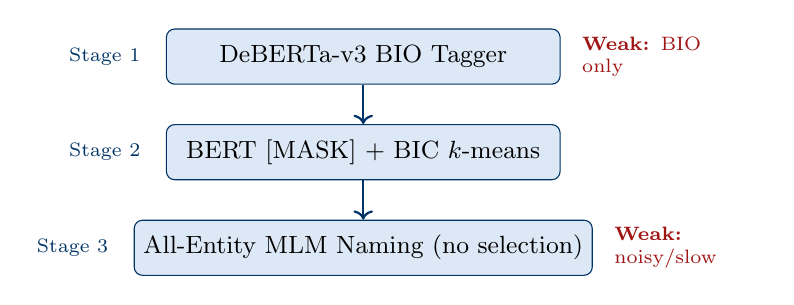
\begin{tikzpicture}[node distance=0.5cm,
          stage/.style={draw=navyblue,fill=lightblue,rounded corners=3pt,
                        minimum width=5cm,minimum height=0.7cm,
                        align=center,font=\small}]
        \node[stage] (md) {DeBERTa-v3 BIO Tagger};
        \node[stage,below=of md] (et) {BERT [MASK] + BIC $k$-means};
        \node[stage,below=of et] (cn) {All-Entity MLM Naming (no selection)};
        \draw[->,thick,navyblue] (md) -- (et);
        \draw[->,thick,navyblue] (et) -- (cn);
        \node[left=0.2cm,font=\scriptsize,navyblue] at (md.west) {Stage 1};
        \node[left=0.2cm,font=\scriptsize,navyblue] at (et.west) {Stage 2};
        \node[left=0.2cm,font=\scriptsize,navyblue] at (cn.west) {Stage 3};
        \node[dkred,font=\scriptsize,right=0.15cm,text width=1.8cm] at (md.east)
          {\textbf{Weak:} BIO only};
        \node[dkred,font=\scriptsize,right=0.15cm,text width=1.8cm] at (cn.east)
          {\textbf{Weak:} noisy/slow};
      \end{tikzpicture}}%
    \end{column}
  \end{columns}
\end{frame}

% ------------------------------------------------------------------
% SLIDE 7 — RESEARCH GAP
% ------------------------------------------------------------------
\begin{frame}{Research Gap \& Thesis Objectives}
  \begin{columns}[T]
    \begin{column}{0.5\textwidth}
      \begin{alertblock}{Gap 1 — Span Detection}
        No open-world NER system uses\\
        \textbf{multi-view} span detection for\\
        cross-domain robustness.
      \end{alertblock}
      \vspace{0.3em}
      \begin{alertblock}{Gap 2 — Entity Typing Efficiency}
        Soft prompt tuning has not been\\
        applied to entity type embedding\\
        learning in open-world NER.
      \end{alertblock}
      \vspace{0.3em}
      \begin{alertblock}{Gap 3 — Exemplar Diversity}
        Centroid-nearest / random exemplar\\
        selection for cluster naming is\\
        sub-optimal and unstable.
      \end{alertblock}
    \end{column}
    \begin{column}{0.5\textwidth}
      \begin{exampleblock}{Overarching Contribution}
        \small
        Build a complete framework: given an \textbf{unannotated target corpus}, automatically produce entity spans each assigned a \textbf{human-readable type name} — no predefined type list, no target-domain labels.
      \end{exampleblock}
      \vspace{0.3em}
      \textbf{Technical Objectives:}
      \begin{enumerate}
        \setlength{\itemsep}{0.3em}
        \small
        \item Integrate \textbf{DTrans multi-view} detection\\(BIO + SE + TB) into the OWNER pipeline
        \item Develop \textbf{two-stage soft-prompt} entity typing\\— better initialization, minimal forgetting
        \item Propose \textbf{MMR-based} exemplar selection\\for more specific, stable cluster naming
      \end{enumerate}
      \vspace{0.3em}
      \begin{block}{Key constraint}
        \textbf{Zero target-domain supervision} at any stage.
      \end{block}
    \end{column}
  \end{columns}
\end{frame}

% =============================================================
\section{Proposed Solution}
% =============================================================

% ------------------------------------------------------------------
% SLIDE 8 — SYSTEM ARCHITECTURE
% ------------------------------------------------------------------
\begin{frame}{Span2Type: System Architecture Overview}
  \begin{columns}[T]
    \begin{column}{0.55\textwidth}
      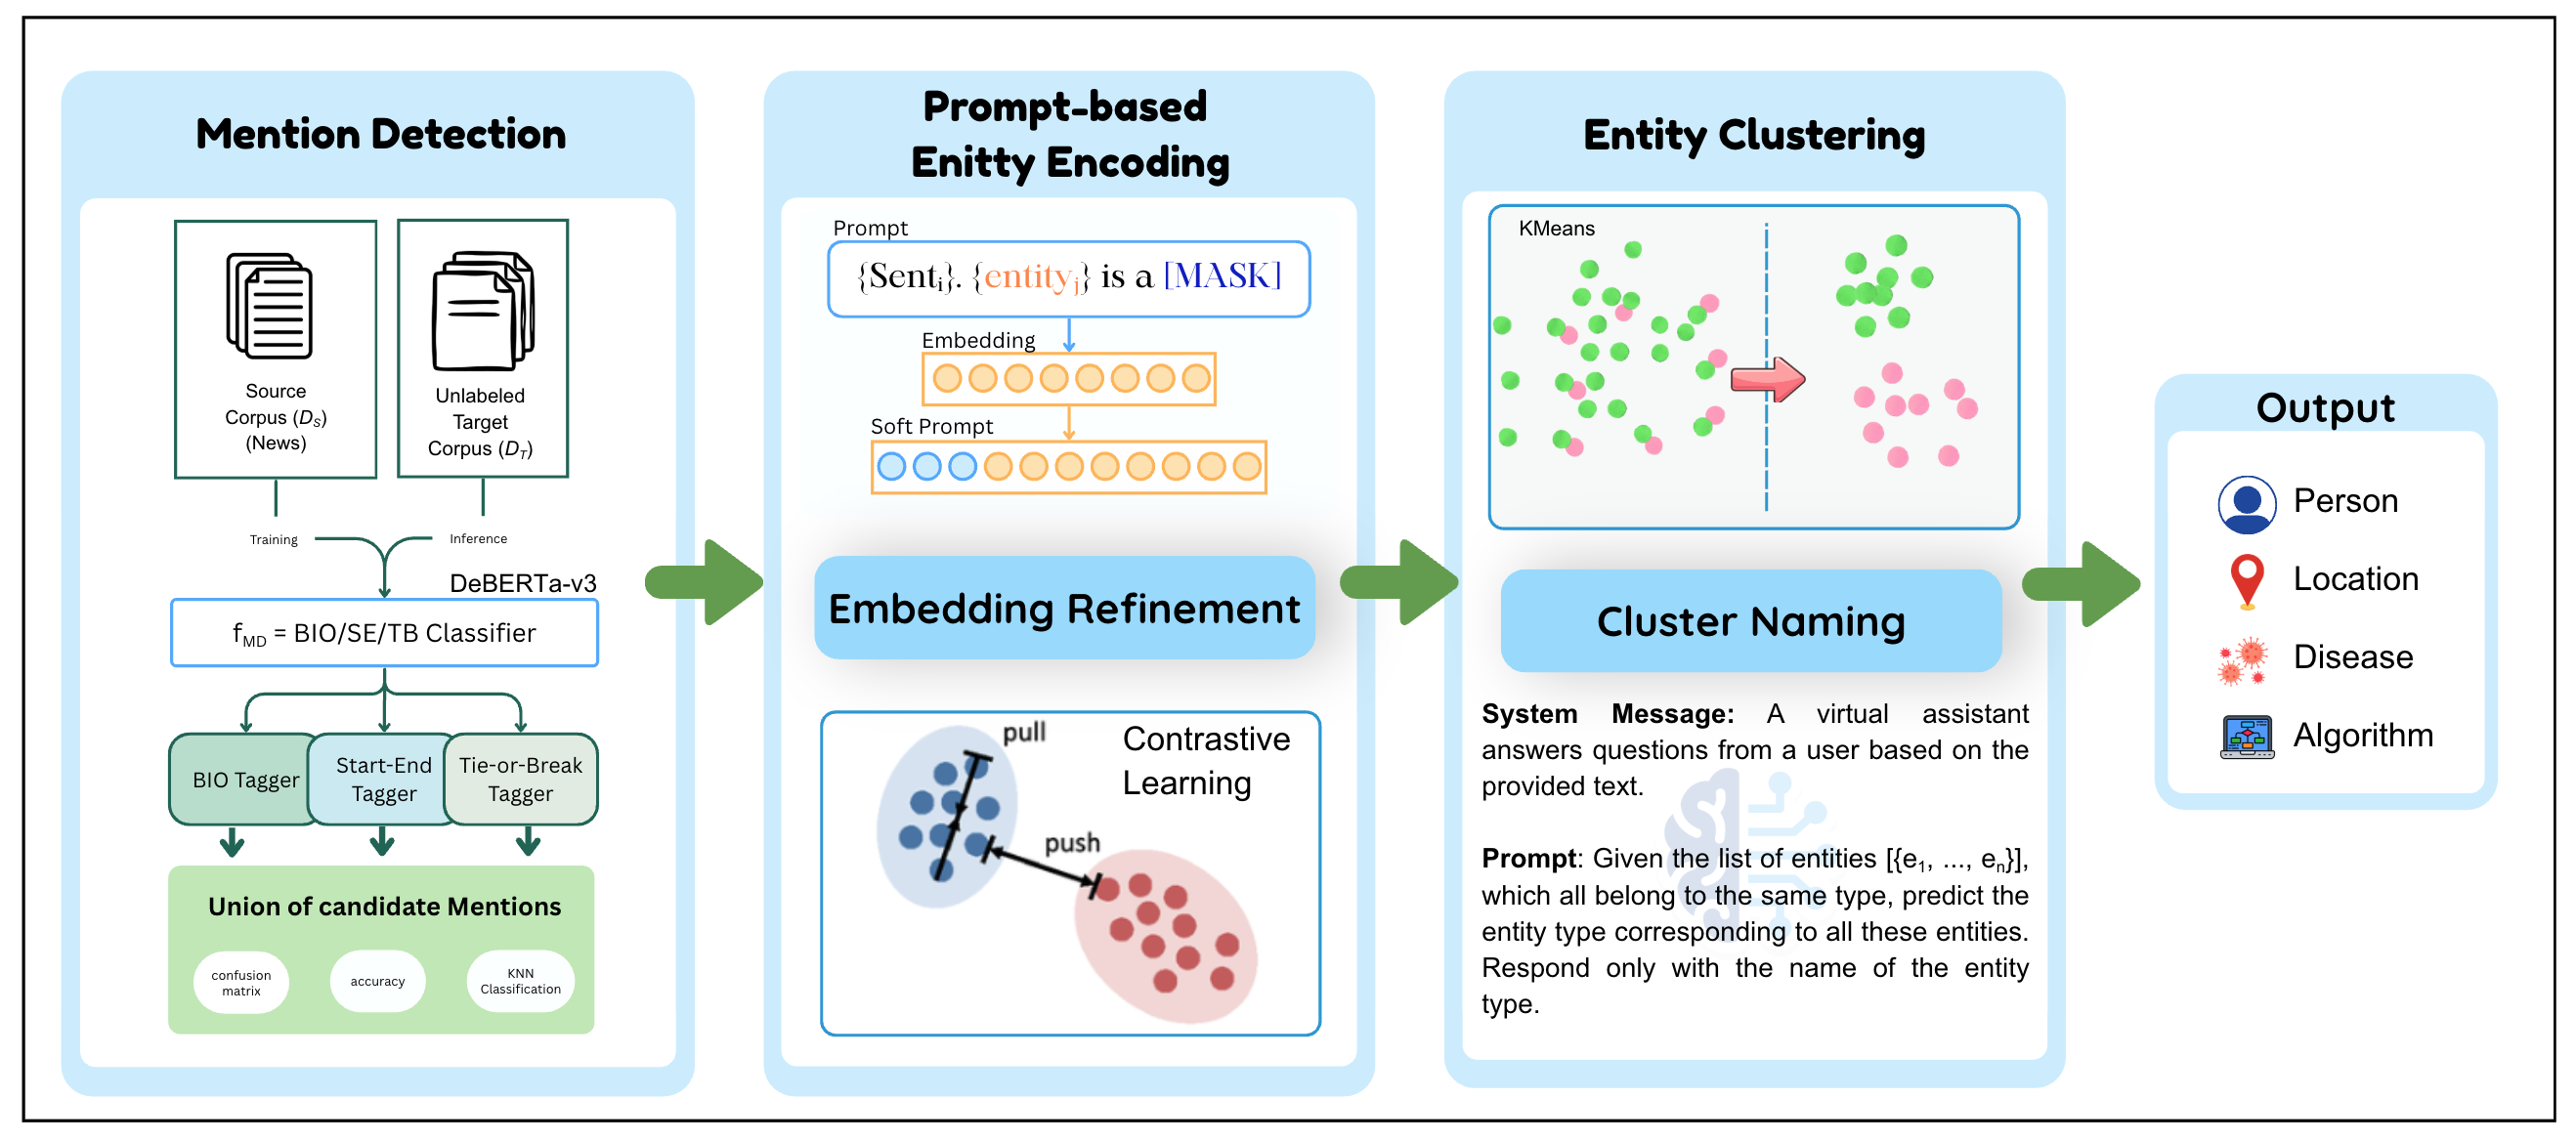
\includegraphics[width=\textwidth]{../figure/Span2Type.png}
    \end{column}
    \begin{column}{0.44\textwidth}
      \textbf{Three-stage pipeline:}
      \vspace{0.3em}
      \begin{enumerate}
        \setlength{\itemsep}{0.5em}
        \item \textbf{Entity Detection}\\
          DTrans: BIO + Start-End +\\Tie-Break decoders\\
          {\small\textit{replaces OWNER's BIO-only tagger}}
        \item \textbf{Entity Typing}\\
          BERT [MASK] template\\
          + soft prompt variant\\
          + BIC $k$-means clustering
        \item \textbf{Cluster Naming}\\
          MMR exemplar selection\\
          + MLM or LLM backend\\
          {\small\textit{replaces all-entity / random}}
      \end{enumerate}
      \vspace{0.4em}
      \begin{block}{Key property}
        \textbf{No target-domain labels} at any stage.
      \end{block}
    \end{column}
  \end{columns}
\end{frame}

% ------------------------------------------------------------------
% SLIDE 9 — CHALLENGES → SOLUTIONS MAP
% ------------------------------------------------------------------
\begin{frame}{Mapping Challenges to Contributions}
  \vspace{-0.3em}
  \begin{block}{\small Framework contribution}
    \small\textbf{Span2Type}: unannotated corpus $\xrightarrow{\text{zero supervision}}$ entity spans + human-readable type list (automatic entity type discovery)
  \end{block}
  \vspace{0.15em}
  \begin{center}
  \small
  \setlength{\tabcolsep}{5pt}
  \renewcommand{\arraystretch}{1.3}
  \begin{tabular}{p{3.3cm}|p{3.3cm}|p{5cm}}
    \toprule
    \textbf{Challenge} & \textbf{Root Cause} & \textbf{Span2Type Solution} \\
    \midrule
    \#1 Robust span detection & BIO sees only one view of entity boundaries & \hb{DTrans}: BIO + Start-End + Tie-Break, jointly with Mean Teaching \\
    \hline
    \#2 Unknown type inventory & Fixed label space in supervised models & \hb{BIC-guided $k$-means} — retained from OWNER \\
    \hline
    \#3 Interpretability gap & Cluster IDs carry no semantic content & \hb{MMR} exemplar selection + \hb{LLM} naming backend \\
    \hline
    \multicolumn{2}{l|}{\textit{Cross-cutting: typing quality}} & \hb{Two-stage soft prompt}: frozen warmup $\to$ full fine-tuning at low LR \\
    \bottomrule
  \end{tabular}
  \end{center}
  \vspace{0.2em}
  \begin{columns}
    \begin{column}{0.6\textwidth}
      \begin{exampleblock}{Pipeline cascade effect}
        Better spans $\to$ cleaner embeddings $\to$\\
        more coherent clusters $\to$ better names
      \end{exampleblock}
    \end{column}
    \begin{column}{0.38\textwidth}
      \small
      \textbf{Improvements compound:}\\
      OWNER: 49.4 avg AMI\\
      \textbf{Span2Type: 61.4 avg AMI}\\
      \hg{$\Delta = +12.0$ points}
    \end{column}
  \end{columns}
\end{frame}

% =============================================================
\section{Methodology}
% =============================================================

% ------------------------------------------------------------------
% SLIDE 10 — STAGE 1 MOTIVATION
% ------------------------------------------------------------------
\begin{frame}{Stage 1 — Multi-View Entity Detection: Motivation}
  \begin{columns}[T]
    \begin{column}{0.5\textwidth}
      \textbf{Why single-view BIO is insufficient:}
      \begin{itemize}
        \item Classifies each token as B/I/O in isolation
        \item Struggles with multi-token technical spans:\\
          \emph{support vector machine}\\
          \emph{convolutional neural network}
        \item One wrong token-tag $\to$ entire span lost
      \end{itemize}
      \vspace{0.5em}
      \textbf{Three complementary views of a span:}
      \begin{enumerate}
        \item \hb{BIO} — global sequential context
        \item \hb{Start-End (SE)} — explicit boundary positions
        \item \hb{Tie-Break (TB)} — pairwise token adjacency
      \end{enumerate}
      \vspace{0.5em}
      \begin{block}{Key insight}
        Union of three views $\to$ \textbf{higher recall}\\
        under domain shift
      \end{block}
    \end{column}
    \begin{column}{0.5\textwidth}
      \small
      \textbf{Example: ``support vector machine''}
      \vspace{0.4em}

      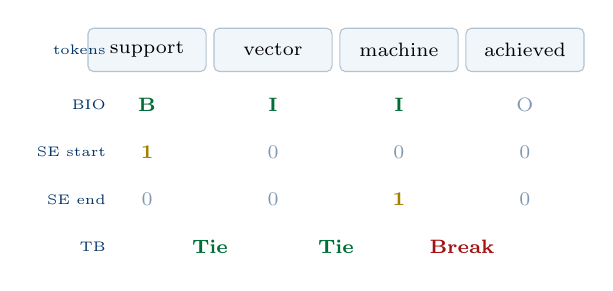
\begin{tikzpicture}[
          tok/.style={draw=navyblue!30,fill=lightblue!40,rounded corners=2pt,
                      minimum width=1.5cm,minimum height=0.55cm,
                      font=\scriptsize,align=center},
          lbl/.style={font=\scriptsize,align=center},
          row/.style={font=\tiny,navyblue}]
        % tokens
        \node[tok] (s) at (0,0)     {support};
        \node[tok] (v) at (1.6,0)   {vector};
        \node[tok] (m) at (3.2,0)   {machine};
        \node[tok] (a) at (4.8,0)   {achieved};
        % BIO
        \node[row,left=0.1cm] at (-0.3,0) {tokens};
        \node[row,left=0.1cm] at (-0.3,-0.7) {BIO};
        \node[row,left=0.1cm] at (-0.3,-1.3) {SE start};
        \node[row,left=0.1cm] at (-0.3,-1.9) {SE end};
        \node[row,left=0.1cm] at (-0.3,-2.5) {TB};
        % BIO row
        \node[lbl,dkgreen] at (0,-0.7)   {\textbf{B}};
        \node[lbl,dkgreen] at (1.6,-0.7) {\textbf{I}};
        \node[lbl,dkgreen] at (3.2,-0.7) {\textbf{I}};
        \node[lbl,navyblue!50] at (4.8,-0.7) {O};
        % SE start
        \node[lbl,gold!80!black] at (0,-1.3) {\textbf{1}};
        \node[lbl,navyblue!50]   at (1.6,-1.3) {0};
        \node[lbl,navyblue!50]   at (3.2,-1.3) {0};
        \node[lbl,navyblue!50]   at (4.8,-1.3) {0};
        % SE end
        \node[lbl,navyblue!50]   at (0,-1.9) {0};
        \node[lbl,navyblue!50]   at (1.6,-1.9) {0};
        \node[lbl,gold!80!black] at (3.2,-1.9) {\textbf{1}};
        \node[lbl,navyblue!50]   at (4.8,-1.9) {0};
        % TB
        \node[lbl,dkgreen]       at (0.8,-2.5)  {\textbf{Tie}};
        \node[lbl,dkgreen]       at (2.4,-2.5)  {\textbf{Tie}};
        \node[lbl,dkred]         at (4.0,-2.5)  {\textbf{Break}};
      \end{tikzpicture}
      \vspace{0.3em}
      \footnotesize
      All three views agree on the same 3-token span.\\
      Even if BIO mislabels one token, SE or TB recovers it.
    \end{column}
  \end{columns}
\end{frame}

% ------------------------------------------------------------------
% SLIDE 11 — DTRANS ARCHITECTURE
% ------------------------------------------------------------------
\begin{frame}{DTrans Multi-View Architecture}
  \begin{columns}[T]
    \begin{column}{0.5\textwidth}
      \textbf{Backbone:} BERT-base-cased (12L, hidden $d=768$)\\
      Input $\mathbf{x}$ $\to$ encoder $\to$ $\mathbf{H} \in \mathbb{R}^{T \times d}$

      \vspace{0.6em}
      \textbf{Three parallel heads:}

      \textit{BIO decoder:}
      \[
        p^{\text{BIO}}_t = \mathrm{softmax}(\mathbf{W}_{\text{bio}}\,\mathbf{h}_t)
      \]
      where $\mathbf{W}_{\text{bio}} \in \mathbb{R}^{3 \times d}$

      \textit{Start-End decoder:}
      \[
        p^{\text{end}}_t = \mathrm{softmax}(\mathbf{W}_{\text{end}}[\mathbf{h}_t;\,\hat{p}^{\text{start}}_t])
      \]
      End conditions on predicted start $\Rightarrow$ boundary coherence

      \textit{Tie-Break decoder:}
      \[
        p^{\text{tb}}_t = \mathrm{softmax}(\mathbf{W}_{\text{tb}}(\mathbf{h}_t + \mathbf{h}_{t+1}))
      \]

      \textbf{Total loss:}
      \[
        \mathcal{L}_{\text{ED}} = \mathcal{L}_{\text{BIO}} + \tfrac{\mathcal{L}_{\text{start}}+\mathcal{L}_{\text{end}}}{2} + \mathcal{L}_{\text{TB}}
      \]
    \end{column}
    \begin{column}{0.5\textwidth}
      \vspace{0.3em}
      \resizebox{0.95\linewidth}{!}{%
      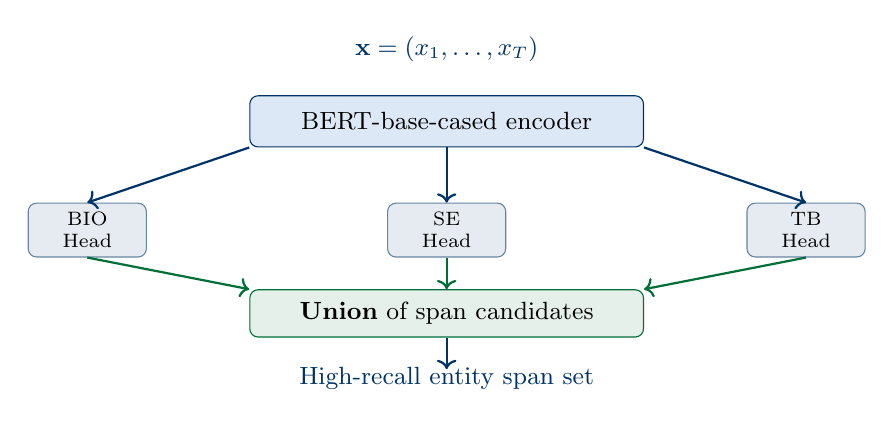
\begin{tikzpicture}[
          enc/.style={draw=navyblue,fill=lightblue,rounded corners=3pt,
                      minimum width=5cm,minimum height=0.65cm,
                      align=center,font=\small},
          head/.style={draw=navyblue!60,fill=navyblue!10,rounded corners=3pt,
                       minimum width=1.5cm,minimum height=0.6cm,
                       align=center,font=\scriptsize},
          merge/.style={draw=dkgreen,fill=dkgreen!10,rounded corners=3pt,
                        minimum width=5cm,minimum height=0.6cm,
                        align=center,font=\small}]
        \node[enc] (bert) {BERT-base-cased encoder};
        \node[head,below left=0.7cm and 1.3cm of bert] (bio) {BIO\\Head};
        \node[head,below=0.7cm of bert] (se) {SE\\Head};
        \node[head,below right=0.7cm and 1.3cm of bert] (tb) {TB\\Head};
        \node[merge,below=1.8cm of bert] (union)
          {\textbf{Union} of span candidates};
        \draw[->,thick,navyblue] (bert.south west) -- (bio.north);
        \draw[->,thick,navyblue] (bert.south) -- (se.north);
        \draw[->,thick,navyblue] (bert.south east) -- (tb.north);
        \draw[->,thick,dkgreen] (bio.south) -- (union.north west);
        \draw[->,thick,dkgreen] (se.south) -- (union.north);
        \draw[->,thick,dkgreen] (tb.south) -- (union.north east);
        \node[above=0.3cm,font=\small,navyblue] at (bert.north) {$\mathbf{x} = (x_1,\ldots,x_T)$};
        \node[below=0.25cm,font=\small,navyblue] at (union.south) {High-recall entity span set};
        \draw[->,thick,navyblue] (union.south) -- ++(0,-0.4cm);
      \end{tikzpicture}}%
      \vspace{0.3em}
      \begin{block}{Mean Teaching (EMA)}
        \footnotesize
        $\tilde{\boldsymbol{\theta}}_t = \alpha\,\tilde{\boldsymbol{\theta}}_{t-1}
          + (1-\alpha)\,\boldsymbol{\theta}_t$\\
        $\alpha=0.995$; soft pseudo-labels $\to$\\
        auxiliary consistency loss
      \end{block}
    \end{column}
  \end{columns}
\end{frame}

% ------------------------------------------------------------------
% SLIDE 12 — ENTITY TYPING TEMPLATE
% ------------------------------------------------------------------
\begin{frame}{Stage 2 — Fill-in-the-Blank Entity Representation}
  \begin{columns}[T]
    \begin{column}{0.5\textwidth}
      \textbf{Template construction:}
      \[
        \underbrace{\texttt{[CLS]}\ x_1\cdots x_T}_{\text{sentence}}\
        \underbrace{m}_{\text{entity}}\ \texttt{is a}\
        \underbrace{\texttt{[MASK]}}_{\text{type}}\ \texttt{.[SEP]}
      \]
      \vspace{-0.3em}
      \begin{itemize}
        \item Repeating the span $m$ gives BERT an explicit type cue
        \item Leverages BERT's cloze pretraining knowledge
      \end{itemize}

      \vspace{0.5em}
      \textbf{Entity embedding:}
      \[
        \mathbf{e}_s = \mathrm{Dropout}(\mathbf{h}_{\texttt{[MASK]}}) \in \mathbb{R}^d
      \]

      \vspace{0.4em}
      \textbf{Training:} Batch Triplet Margin Loss
      \[
        \mathcal{L} = \tfrac{1}{|\mathcal{T}|}\sum_{(i,j,k)\in\mathcal{T}}
        \max(0,\; d_{ij} - d_{ik} + \gamma)
      \]
      $\gamma=1.0$; triplet $(i,j,k)$: same type $(i,j)$,\; diff type $(i,k)$
    \end{column}
    \begin{column}{0.48\textwidth}
      \begin{exampleblock}{Concrete Example}
        \small
        \textbf{Sentence:} \textit{Albert Einstein was born in Germany}\\
        \textbf{Span:} \textit{Albert Einstein}\\[5pt]
        \textbf{Template:}\\
        \texttt{[CLS] Albert Einstein was born}\\
        \texttt{in Germany \hl{Albert Einstein}}\\
        \texttt{is a \textbf{[MASK]} . [SEP]}\\[5pt]
        BERT predicts: \hg{\textit{physicist}}, \hg{\textit{scientist}}\\[5pt]
        $\mathbf{e}_s$ = [MASK] hidden state\\
        $\to$ rich type-semantic representation
      \end{exampleblock}
      \vspace{0.4em}
      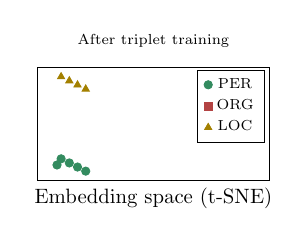
\begin{tikzpicture}[scale=0.75]
        \begin{axis}[
          xlabel={Embedding space (t-SNE)},
          ylabel={},
          xtick=\empty, ytick=\empty,
          width=5.5cm, height=3.5cm,
          axis lines=box,
          title={\scriptsize After triplet training},
          title style={font=\scriptsize}]
          \addplot[only marks,mark=*,mark size=2pt,
                   color=dkgreen!80] coordinates {
            (1,1)(1.2,0.8)(0.9,1.1)(1.1,0.9)(0.85,0.95)};
          \addplot[only marks,mark=square*,mark size=2pt,
                   color=dkred!80] coordinates {
            (3,3)(3.2,2.8)(2.9,3.1)(3.1,2.9)(2.85,2.95)};
          \addplot[only marks,mark=triangle*,mark size=2pt,
                   color=gold!80!black] coordinates {
            (1,3)(1.2,2.8)(0.9,3.1)(1.1,2.9)};
          \legend{\scriptsize PER,\scriptsize ORG,\scriptsize LOC}
        \end{axis}
      \end{tikzpicture}
    \end{column}
  \end{columns}
\end{frame}

% ------------------------------------------------------------------
% SLIDE 13 — SOFT PROMPT
% ------------------------------------------------------------------
\begin{frame}{Soft Prompt Variant — 3,840 vs.\ 110 Million Parameters}
  \begin{columns}[T]
    \begin{column}{0.5\textwidth}
      \textbf{Full fine-tuning problem:}
      \begin{itemize}
        \item Updates all $\sim$110M BERT parameters
        \item Risk of catastrophic forgetting of\\pretrained world knowledge
        \item Cross-domain: frozen backbone is safer
      \end{itemize}
      \vspace{0.5em}
      \textbf{Soft prompt (P-tuning / Prefix-tuning):}
      \begin{itemize}
        \item $N_p = 5$ trainable tokens $\mathbf{P} \in \mathbb{R}^{N_p \times d}$
        \item Prepended to template embeddings:
      \end{itemize}
      \[
        \text{inputs} = [\,\underbrace{\mathbf{P}}_{\text{trainable}};\;
                            \underbrace{\mathbf{E}_{\mathbf{x}}}_{\text{frozen}}\,]
        \in \mathbb{R}^{(N_p+L)\times d}
      \]
      \begin{itemize}
        \item BERT backbone: \textbf{strictly frozen}
        \item Trainable params: $5\times768 = \mathbf{3{,}840}$
        \item [MASK] index shifted by $N_p$
      \end{itemize}
    \end{column}
    \begin{column}{0.5\textwidth}
      \resizebox{\linewidth}{!}{%
      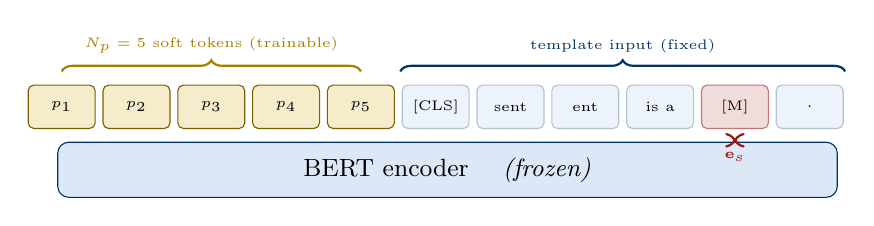
\begin{tikzpicture}[
          tok/.style={draw=navyblue!30,fill=lightblue!50,rounded corners=2pt,
                      minimum width=0.85cm,minimum height=0.55cm,
                      font=\tiny,align=center},
          ptok/.style={draw=gold!60!black,fill=gold!20,rounded corners=2pt,
                       minimum width=0.85cm,minimum height=0.55cm,
                       font=\tiny,align=center}]
        \node[ptok] (p1) at (0,0)    {$p_1$};
        \node[ptok] (p2) at (0.95,0) {$p_2$};
        \node[ptok] (p3) at (1.9,0)  {$p_3$};
        \node[ptok] (p4) at (2.85,0) {$p_4$};
        \node[ptok] (p5) at (3.8,0)  {$p_5$};
        \node[tok] at (4.75,0)  {[CLS]};
        \node[tok] at (5.7,0)   {sent};
        \node[tok] at (6.65,0)  {ent};
        \node[tok] at (7.6,0)   {is a};
        \node[tok,draw=dkred!60,fill=dkred!15] at (8.55,0) {[M]};
        \node[tok] at (9.5,0)   {.};
        \draw[decorate,decoration={brace,amplitude=4pt},gold!80!black,thick]
          (0,0.45) -- (3.8,0.45) node[midway,above=3pt,font=\tiny,gold!80!black]
          {$N_p=5$ soft tokens (trainable)};
        \draw[decorate,decoration={brace,amplitude=4pt},navyblue,thick]
          (4.3,0.45) -- (9.95,0.45) node[midway,above=3pt,font=\tiny,navyblue]
          {template input (fixed)};
        \node[draw=navyblue,fill=lightblue,rounded corners,
              minimum width=9.9cm,minimum height=0.7cm,
              font=\small,align=center] at (4.9,-0.8)
          {BERT encoder \quad\textit{(frozen)}};
        \draw[<->,dkred,thick,dashed] (8.55,-0.4) -- (8.55,-0.45)
          node[below,font=\tiny,dkred] {$\mathbf{e}_s$};
      \end{tikzpicture}}%
      \vspace{0.4em}
      \begin{block}{Parameter comparison}
        \footnotesize
        \begin{tabular}{lr}
          Full BERT fine-tuning & $\sim$110,000,000 \\
          \textbf{Soft prompt only} & \textbf{3,840} \\
          Reduction & $\times$28,645 \\
        \end{tabular}
      \end{block}
    \end{column}
  \end{columns}
\end{frame}

% ------------------------------------------------------------------
% SLIDE 14 — TWO-STAGE TRAINING
% ------------------------------------------------------------------
\begin{frame}{Two-Stage Prompt-Initialized Fine-Tuning}
  \begin{columns}[T]
    \begin{column}{0.5\textwidth}
      \textbf{Problem:}
      \begin{itemize}
        \item Soft-only $\to$ limited expressiveness
        \item Full fine-tuning from epoch 1 $\to$ catastrophic forgetting
      \end{itemize}

      \vspace{0.4em}
      \textbf{Solution: two-stage schedule at $E_{\text{unfreeze}}=10$}

      \vspace{0.4em}
      \small
      \setlength{\tabcolsep}{4pt}
      \renewcommand{\arraystretch}{1.3}
      \begin{tabular}{l|cc}
        \toprule
        & \textbf{Stage 1} & \textbf{Stage 2} \\
        & Epochs 1--9 & Epochs 10--30 \\
        \midrule
        Trainable & prompt only & prompt + BERT \\
        LR (prompt) & $3\times10^{-3}$ & $3\times10^{-3}$ \\
        LR (BERT) & frozen & $1\times10^{-5}$ \\
        PLM frozen & \cmark & \xmark \\
        \bottomrule
      \end{tabular}

      \vspace{0.5em}
      \textbf{Critical implementation details:}
      \begin{itemize}
        \item \texttt{add\_param\_group()} — preserves optimizer moments for soft tokens
        \item LR scheduler \textbf{reset} at epoch 10 — PLM LR decays from full value
      \end{itemize}
    \end{column}
    \begin{column}{0.5\textwidth}
      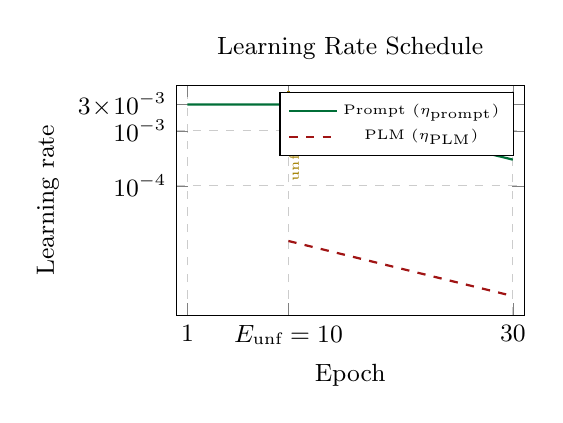
\begin{tikzpicture}
        \begin{axis}[
          width=6cm, height=4.5cm,
          xlabel={Epoch},
          ylabel={Learning rate},
          xmin=0, xmax=31,
          ymin=0,
          xtick={1,10,30},
          xticklabels={1,$E_{\text{unf}}=10$,30},
          ytick={0.0001, 0.001, 0.003},
          yticklabels={$10^{-4}$,$10^{-3}$,$3\!\times\!10^{-3}$},
          ymode=log,
          grid=major,
          grid style={dashed,gray!40},
          legend pos=north east,
          legend style={font=\tiny},
          title={\small Learning Rate Schedule}]
          % Prompt LR - high in stage 1, maintained in stage 2
          \addplot[dkgreen,thick] coordinates {(1,0.003)(9,0.003)(10,0.003)(30,0.0003)};
          \addlegendentry{Prompt ($\eta_{\text{prompt}}$)}
          % PLM LR - zero in stage 1, low in stage 2
          \addplot[dkred,thick,dashed] coordinates {(1,0)(9,0)(10,0.00001)(30,0.000001)};
          \addlegendentry{PLM ($\eta_{\text{PLM}}$)}
          % Vertical dashed line at epoch 10
          \draw[gold!80!black,thick,dashed] (axis cs:10,0) -- (axis cs:10,0.004);
          \node[font=\tiny,gold!80!black,rotate=90] at (axis cs:10.5,0.0005) {unfreeze};
        \end{axis}
      \end{tikzpicture}
      \vspace{0.2em}
      \begin{exampleblock}{Why this works}
        \small
        Stage 1: prompt warms up rapidly ($3\times10^{-3}$)\\
        without disturbing pretrained BERT.\\[3pt]
        Stage 2: BERT adapts at $1\times10^{-5}$ — 300$\times$ smaller —\\
        preserving pretrained representations.
      \end{exampleblock}
    \end{column}
  \end{columns}
\end{frame}

% ------------------------------------------------------------------
% SLIDE 15 — BIC CLUSTERING
% ------------------------------------------------------------------
\begin{frame}{BIC-Guided Automatic Cluster Count}
  \begin{columns}[T]
    \begin{column}{0.5\textwidth}
      \textbf{Challenge:} target domain has \emph{unknown} $k$\\[0.4em]
      \textbf{AutoKmeans:} search $k \in [2, 30]$, step $2$

      \vspace{0.4em}
      \textbf{Bayesian Information Criterion:}
      \[
        \text{BIC}(k) = n \cdot \log\!\Bigl(\tfrac{\mathcal{I}(k)}{n}\Bigr) + \log(n)\cdot k
      \]
      \begin{itemize}
        \item $\mathcal{I}(k)$: inertia (sum of squared distances)
        \item First term: fit quality — decreases with $k$
        \item Second term: complexity penalty — grows with $k$
      \end{itemize}
      \[
        k^* = \arg\min_{k} \text{BIC}(k)
      \]
      \begin{itemize}
        \item k-means++ init, 10 random restarts per $k$
        \item \textbf{Retained unchanged from OWNER}
      \end{itemize}
    \end{column}
    \begin{column}{0.5\textwidth}
      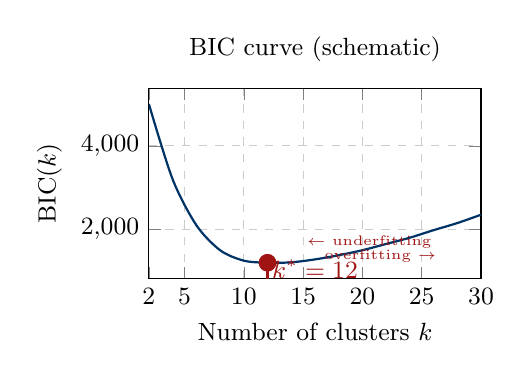
\begin{tikzpicture}
        \begin{axis}[
          width=5.8cm, height=4cm,
          xlabel={Number of clusters $k$},
          ylabel={BIC$(k)$},
          xmin=2, xmax=30,
          xtick={2,5,10,15,20,25,30},
          grid=major, grid style={dashed,gray!40},
          title={\small BIC curve (schematic)}]
          \addplot[navyblue,thick,smooth] coordinates {
            (2,5000)(4,3200)(6,2100)(8,1500)(10,1250)
            (12,1200)(14,1210)(16,1280)(18,1380)
            (20,1500)(22,1650)(24,1800)(26,1980)(28,2150)(30,2350)};
          \addplot[only marks,mark=*,mark size=3pt,dkred]
            coordinates {(12,1200)};
          \node[font=\small,dkred] at (axis cs:16,1050) {$k^*=12$};
          \draw[dkred,dashed,thick] (axis cs:12,800) -- (axis cs:12,1200);
          \node[font=\tiny,dkred,anchor=west] at (axis cs:14.5,1700)
            {$\leftarrow$ underfitting};
          \node[font=\tiny,dkred,anchor=west] at (axis cs:16,1350)
            {overfitting $\rightarrow$};
        \end{axis}
      \end{tikzpicture}
      \vspace{0.2em}
      \small
      After $k^*$ is selected, embeddings $\{\mathbf{e}_s\}$ are assigned cluster labels $c_s \in \{1,\ldots,k^*\}$ for all target-domain spans.
    \end{column}
  \end{columns}
\end{frame}

% ------------------------------------------------------------------
% SLIDE 16 — MMR NAMING
% ------------------------------------------------------------------
\begin{frame}{Stage 3 — MMR-Based Cluster Naming}
  \begin{columns}[T]
    \begin{column}{0.5\textwidth}
      \textbf{Problem with centroid-nearest selection:}
      \begin{itemize}
        \item 16 exemplars all near centroid $\to$ redundant
        \item Single surface form repeated $\to$ unstable naming
      \end{itemize}

      \vspace{0.4em}
      \textbf{Maximal Marginal Relevance (MMR):}
      \[
        \text{MMR}(s) = \lambda \cdot \cos(\mathbf{e}_s,\boldsymbol{\mu}_c)
        - (1{-}\lambda)\cdot \max_{r\in\mathcal{R}} \cos(\mathbf{e}_s,\mathbf{e}_r)
      \]
      \begin{itemize}
        \item First term: \textbf{relevance} to cluster centroid $\boldsymbol{\mu}_c$
        \item Second term: \textbf{diversity} from already-selected $\mathcal{R}$
        \item $\lambda = 0.7$: slightly favours relevance over diversity
        \item Iterate until $|\mathcal{R}| = K_e = 16$
      \end{itemize}

      \begin{block}{Effect}
        Exemplars cover the \textbf{full semantic spread}\\
        of the cluster, not just the centroid cloud
      \end{block}
    \end{column}
    \begin{column}{0.5\textwidth}
      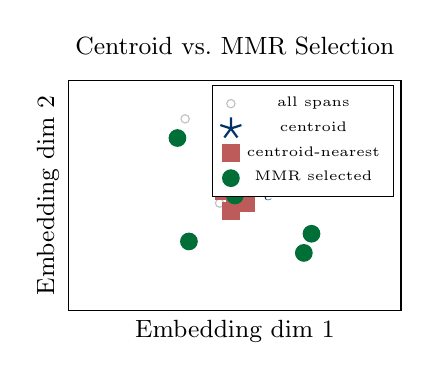
\begin{tikzpicture}
        \begin{axis}[
          width=5.8cm, height=4.5cm,
          xlabel={Embedding dim 1},
          ylabel={Embedding dim 2},
          xmin=-1, xmax=5, ymin=-1, ymax=5,
          xtick=\empty, ytick=\empty,
          axis equal,
          title={\small Centroid vs.\ MMR Selection}]
          % Cluster points (many)
          \addplot[only marks,mark=o,mark size=1.5pt,gray!50]
            coordinates {
              (2,2)(2.3,1.8)(1.7,2.1)(2.1,2.4)(1.9,1.6)
              (2.4,2.2)(1.6,1.8)(2.2,1.7)(0.5,3.5)(4,1)
              (3.5,3.8)(0.8,0.8)(3.8,0.5)(0.7,4)(4.2,3.5)};
          % Centroid
          \addplot[only marks,mark=star,mark size=4pt,navyblue,thick]
            coordinates {(2,2)};
          \node[font=\tiny,navyblue,right=2pt] at (axis cs:2,2) {$\boldsymbol{\mu}_c$};
          % Centroid-nearest (clustered)
          \addplot[only marks,mark=square*,mark size=3pt,dkred!70]
            coordinates {(2,2)(2.3,1.8)(1.7,2.1)(2.1,2.4)(1.9,1.6)(2.4,2.2)};
          % MMR selection (spread)
          \addplot[only marks,mark=*,mark size=3pt,dkgreen]
            coordinates {(2,2)(0.5,3.5)(4,1)(3.5,3.8)(0.8,0.8)(3.8,0.5)};
          \legend{\tiny all spans,\tiny centroid,\tiny centroid-nearest,\tiny MMR selected}
        \end{axis}
      \end{tikzpicture}
      \footnotesize MMR (green) covers the cluster periphery;\\
      centroid-nearest (red) is redundant.
    \end{column}
  \end{columns}
\end{frame}

% ------------------------------------------------------------------
% SLIDE 17 — MLM vs LLM BACKENDS
% ------------------------------------------------------------------
\begin{frame}{Two Naming Backends: MLM and LLM}
  \begin{columns}[T]
    \begin{column}{0.5\textwidth}
      \begin{block}{MLM Backend (BERT)}
        \small
        Template:\\
        \texttt{In this sentence, \{ent\} is a [MASK]. Sentence: \{text\}.}\\[4pt]
        Average vocab distributions over $K_e$ exemplars:
        \[
          \bar{p}_v = \tfrac{1}{K_e}\textstyle\sum_r p_v^{(r)}
        \]
        Post-filter: remove subwords, stopwords, punctuation.\\[4pt]
        \textbf{Output: single token}\\
        \hg{\textit{conference}, \textit{band}, \textit{protein}}\\[4pt]
        \hr{Cannot express compound types:\\
        \textit{musical artist}, \textit{literary genre}}
      \end{block}
    \end{column}
    \begin{column}{0.5\textwidth}
      \begin{block}{LLM Backend (Llama-3 via Ollama)}
        \small
        Two-turn prompt:\\
        \textbf{Sys:} \textit{A virtual assistant answers questions\ldots}\\
        \textbf{User:} \textit{Given entities $\{e_1,\ldots,e_{16}\}$, all of the same type, predict the entity type. Respond only with the type name.}\\[4pt]
        Temperature = 0 (deterministic).\\
        Post-process: $\leq$3 words, lowercase, strip fillers.\\[4pt]
        \textbf{Output: multi-word labels}\\
        \hg{\textit{political party}, \textit{research institute}}\\[4pt]
        \hg{Immune to MLM hallucination artefact}
      \end{block}
    \end{column}
  \end{columns}
  \vspace{0.4em}
  \begin{center}
    \small
    \begin{tabular}{lccc}
      \toprule
      & \textbf{Multi-word output} & \textbf{No hallucination} & \textbf{Avg BERTScore-F1} \\
      \midrule
      MLM (MMR) & \xmark & \xmark & 0.896 \\
      \textbf{LLM (MMR)} & \cmark & \cmark & \textbf{0.956} \\
      \bottomrule
    \end{tabular}
  \end{center}
\end{frame}

% =============================================================
\section{Experiments \& Results}
% =============================================================

% ------------------------------------------------------------------
% SLIDE 18 — EXPERIMENTAL SETUP
% ------------------------------------------------------------------
\begin{frame}{Experimental Setup}
  \begin{columns}[T]
    \begin{column}{0.5\textwidth}
      \textbf{Source training data:}
      \vspace{0.2em}
      \begin{itemize}
        \item \textbf{CoNLL-2003}: English newswire, 4 types, 14k sentences
        \item \textbf{Pile-NER}: diverse web corpus, $\sim$13k types, 50k sentences
      \end{itemize}

      \vspace{0.5em}
      \textbf{Target evaluation (CrossNER):}
      \vspace{0.2em}
      \footnotesize
      \begin{tabular}{lcc}
        \toprule
        Domain & \#Test & \#GT Types \\
        \midrule
        AI           & 431 & 14 \\
        Literature   & 416 & 12 \\
        Music        & 465 & 13 \\
        Politics     & 650 &  9 \\
        Science      & 543 & 17 \\
        \bottomrule
      \end{tabular}
      \vspace{0.3em}
      \normalsize
      \begin{alertblock}{}
        \small Gold labels used \textbf{only for evaluation} — never seen during training or clustering.
      \end{alertblock}
    \end{column}
    \begin{column}{0.48\textwidth}
      \textbf{Key hyperparameters:}
      \vspace{0.3em}
      \footnotesize
      \setlength{\tabcolsep}{4pt}
      \begin{tabular}{ll}
        \toprule
        \textbf{Component} & \textbf{Setting} \\
        \midrule
        Detector backbone & BERT-base-cased \\
        Detector LR       & $1\times10^{-5}$, 50 epochs \\
        EMA decay         & $\alpha = 0.995$ \\
        \midrule
        Typing backbone   & BERT-base-uncased \\
        Full FT LR        & $2\times10^{-5}$, 30 epochs \\
        Soft prompt $N_p$ & 5 tokens \\
        Stage 1 LR        & $3\times10^{-3}$, 10 epochs \\
        Stage 2 LR        & $1\times10^{-5}$, 20 epochs \\
        Triplet margin    & $\gamma = 1.0$ \\
        \midrule
        Clustering range  & $k\in[2,30]$, step 2 \\
        k-means restarts  & 10 per $k$ \\
        \midrule
        MMR exemplars     & $K_e=16$, $\lambda=0.7$ \\
        LLM               & Llama-3 via Ollama \\
        \bottomrule
      \end{tabular}
    \end{column}
  \end{columns}
\end{frame}

% ------------------------------------------------------------------
% SLIDE 19 — EVALUATION METRICS
% ------------------------------------------------------------------
\begin{frame}{Evaluation Metrics — One per Pipeline Stage}
  \begin{columns}[T]
    \begin{column}{0.32\textwidth}
      \begin{block}{Stage 1 — Detection}
        \textbf{Span F1} (exact match)\\[5pt]
        Precision, Recall, F1 at\\
        the span level on test set.\\[5pt]
        Measures whether DTrans\\
        transfers better than BIO.
      \end{block}
    \end{column}
    \begin{column}{0.32\textwidth}
      \begin{block}{Stage 2 — Typing}
        \textbf{AMI} (Adjusted Mutual\\Information)\\[5pt]
        \textit{Mapping-free:} no\\cluster-to-type assignment.\\[5pt]
        Robust to permutations,\\over-seg., over-merging.\\[5pt]
        0 = random, 1 = perfect.
      \end{block}
    \end{column}
    \begin{column}{0.32\textwidth}
      \begin{block}{Stage 3 — Naming}
        \textbf{BERTScore-F1}\\(RoBERTa-large)\\[5pt]
        Semantic similarity of\\predicted vs.\ gold type name.\\[5pt]
        Partial credit for\\semantically close labels.
      \end{block}
    \end{column}
  \end{columns}
  \vspace{0.5em}
  \begin{columns}
    \begin{column}{0.5\textwidth}
      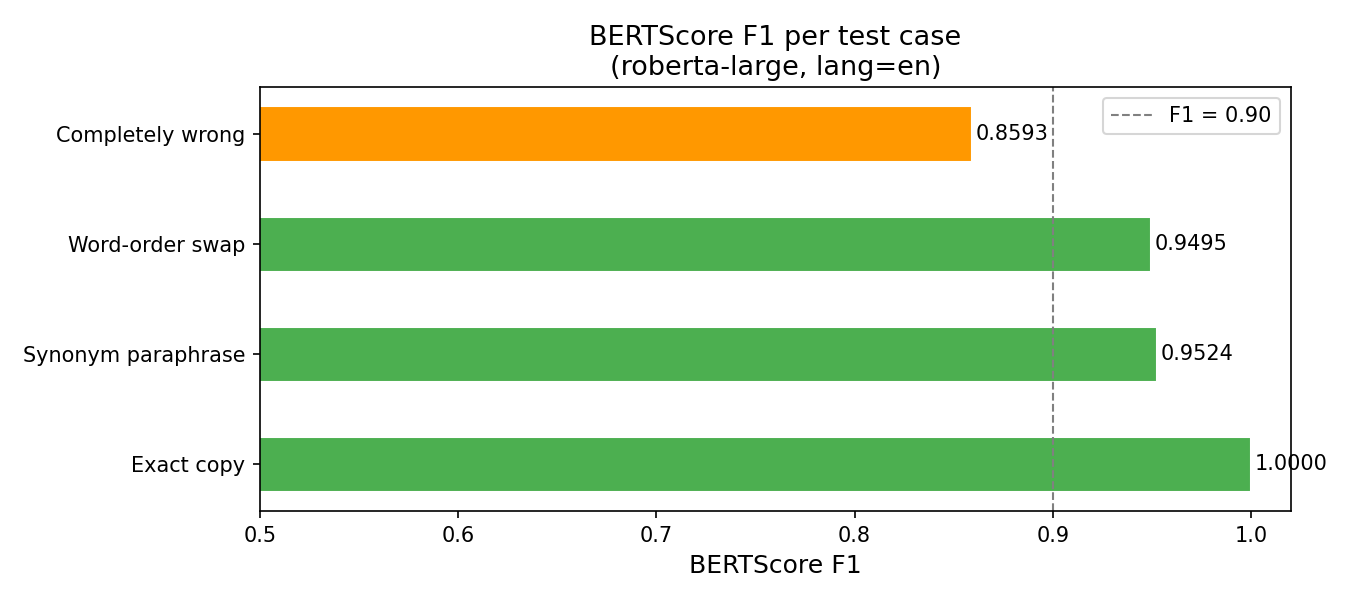
\includegraphics[width=\textwidth]{../figure/bertscore_bar.png}
    \end{column}
    \begin{column}{0.48\textwidth}
      \small
      \textbf{BERTScore interpretation:}\\[3pt]
      Meaningful range is \textbf{0.86–1.0}\\
      (even a wrong label scores $\approx$0.86\\
      due to shared embedding space).\\[5pt]
      Exact copy $= 1.0$\\
      Synonym paraphrase $\approx 0.95$\\
      Related concept $\approx 0.90$\\
      Wrong prediction $\approx 0.86$
    \end{column}
  \end{columns}
\end{frame}

% ------------------------------------------------------------------
% SLIDE 20 — MAIN RESULTS
% ------------------------------------------------------------------
\begin{frame}{Main Results: End-to-End AMI on CrossNER}
  \begin{columns}[T]
    \begin{column}{0.5\textwidth}
      \footnotesize
      \setlength{\tabcolsep}{3.5pt}
      \renewcommand{\arraystretch}{1.2}
      \begin{tabular}{l|ccccc|c}
        \toprule
        \textbf{Method} & AI & Lit & Mus & Pol & Sci & \textbf{Avg} \\
        \midrule
        \multicolumn{7}{l}{\textit{Unsupervised Baselines}} \\
        ChatIE (GPT-4o) & 21.8 & 37.5 & 43.7 & 37.2 & 35.0 & 35.0 \\
        UniNER         & 33.5 & 42.8 & 48.1 & 40.3 & 43.7 & 41.7 \\
        UniNER (GPT-4o)& 36.7 & 49.8 & 53.6 & 48.8 & 48.1 & 47.4 \\
        OWNER (CoNLL)  & 44.3 & 46.6 & 50.1 & 53.7 & 52.3 & 49.4 \\
        OWNER (Pile)   & 39.4 & 49.5 & 52.5 & 48.5 & 50.9 & 48.2 \\
        \midrule
        \multicolumn{7}{l}{\textit{Proposed}} \\
        Span2Type (Pile) & 50.0 & 52.8 & 56.2 & 55.8 & 62.3 & 55.4 \\
        \rowcolor{gold!25}
        \textbf{Span2Type (CoNLL)} & \textbf{57.6} & \textbf{56.9} & \textbf{60.0} & \textbf{66.3} & \textbf{66.0} & \textbf{61.4} \\
        \bottomrule
      \end{tabular}
      \vspace{0.4em}
      \normalsize
      \begin{exampleblock}{Key numbers}
        vs.\ OWNER: \hg{$+$12.0 pts} avg AMI\\
        vs.\ best LLM baseline (UniNER GPT-4o): \hg{$+$14.0 pts}
      \end{exampleblock}
    \end{column}
    \begin{column}{0.5\textwidth}
      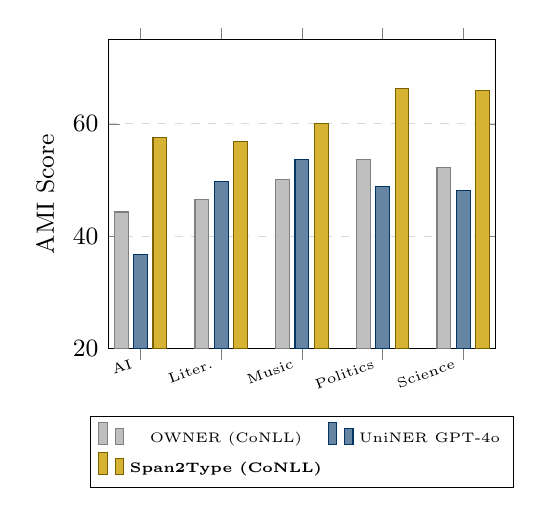
\begin{tikzpicture}
        \begin{axis}[
          ybar, bar width=5pt,
          width=6.5cm, height=5.5cm,
          ylabel={AMI Score},
          symbolic x coords={AI,Liter.,Music,Politics,Science},
          xtick=data,
          x tick label style={font=\tiny,rotate=20,anchor=east},
          ymin=20, ymax=75,
          legend style={at={(0.5,-0.22)},anchor=north,
                        legend columns=2,font=\tiny},
          ymajorgrids=true,
          grid style={dashed,gray!30}]
          \addplot[fill=gray!50,draw=gray] coordinates {
            (AI,44.3)(Liter.,46.6)(Music,50.1)(Politics,53.7)(Science,52.3)};
          \addplot[fill=navyblue!60,draw=navyblue] coordinates {
            (AI,36.7)(Liter.,49.8)(Music,53.6)(Politics,48.8)(Science,48.1)};
          \addplot[fill=gold!80,draw=gold!60!black] coordinates {
            (AI,57.6)(Liter.,56.9)(Music,60.0)(Politics,66.3)(Science,66.0)};
          \legend{OWNER (CoNLL), UniNER GPT-4o, \textbf{Span2Type (CoNLL)}}
        \end{axis}
      \end{tikzpicture}
    \end{column}
  \end{columns}
\end{frame}

% ------------------------------------------------------------------
% SLIDE 21 — ENTITY DETECTION RESULTS
% ------------------------------------------------------------------
\begin{frame}{Entity Detection F1: Multi-View vs.\ Single-View}
  \begin{columns}[T]
    \begin{column}{0.5\textwidth}
      \footnotesize
      \setlength{\tabcolsep}{3pt}
      \renewcommand{\arraystretch}{1.2}
      \begin{tabular}{l|ccccc|c}
        \toprule
        \textbf{Model} & AI & Lit & Mus & Pol & Sci & \textbf{Avg} \\
        \midrule
        PURE       & 39.8 & 37.1 & 33.8 & 32.4 & 35.7 & 35.8 \\
        SpanProto  & 54.1 & 62.9 & 59.6 & 68.7 & 59.7 & 61.0 \\
        WL-Coref   & 57.4 & 68.3 & 66.9 & 72.1 & 63.4 & 65.6 \\
        BIO (OWNER)& 60.5 & \textbf{83.9} & 79.0 & 80.6 & 74.4 & 75.7 \\
        \rowcolor{gold!25}
        \textbf{BIO-SE-TB} & \textbf{81.4} & 82.7 & \textbf{82.7} & \textbf{89.6} & \textbf{75.4} & \textbf{82.4} \\
        \bottomrule
      \end{tabular}
      \vspace{0.3em}
      \normalsize
      \begin{block}{Average gain}
        OWNER BIO: 75.68\\
        DTrans BIO-SE-TB: \textbf{82.35}\\
        Improvement: \hg{$+6.67$ F1 points}
      \end{block}
    \end{column}
    \begin{column}{0.5\textwidth}
      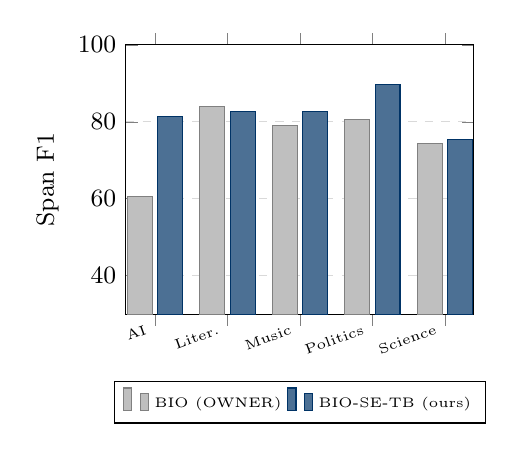
\begin{tikzpicture}
        \begin{axis}[
          ybar, bar width=9pt,
          width=6cm, height=5cm,
          ylabel={Span F1},
          symbolic x coords={AI,Liter.,Music,Politics,Science},
          xtick=data,
          x tick label style={font=\tiny,rotate=20,anchor=east},
          ymin=30, ymax=100,
          legend style={at={(0.5,-0.25)},anchor=north,
                        legend columns=2,font=\tiny},
          ymajorgrids=true,
          grid style={dashed,gray!30},
          ]
          \addplot[fill=gray!50,draw=gray] coordinates {
            (AI,60.5)(Liter.,83.9)(Music,79.0)(Politics,80.6)(Science,74.4)};
          \addplot[fill=navyblue!70,draw=navyblue] coordinates {
            (AI,81.4)(Liter.,82.7)(Music,82.7)(Politics,89.6)(Science,75.4)};
          \legend{BIO (OWNER), BIO-SE-TB (ours)}
        \end{axis}
      \end{tikzpicture}
      \vspace{0.2em}
      \footnotesize
      \hr{Literature regression: $-1.22$} — literary entities\\
      (character names, book titles) follow predictable\\
      proper-noun patterns; SE/TB add noise, not signal.
    \end{column}
  \end{columns}
\end{frame}

% ------------------------------------------------------------------
% SLIDE 22 — NAMING RESULTS
% ------------------------------------------------------------------
\begin{frame}{Cluster Naming: BERTScore-F1 Results}
  \begin{columns}[T]
    \begin{column}{0.5\textwidth}
      \footnotesize
      \setlength{\tabcolsep}{3pt}
      \renewcommand{\arraystretch}{1.2}
      \begin{tabular}{l|ccccc|c}
        \toprule
        \textbf{Method} & AI & Lit & Mus & Pol & Sci & \textbf{Avg} \\
        \midrule
        \#Clusters & 14 & 14 & 22 & 24 & 22 & -- \\
        \#GT Types & 14 & 12 & 13 &  9 & 17 & -- \\
        \midrule
        OWNER MLM & \textbf{.989} & .974 & \textbf{.958} & \textbf{.964} & .945 & .966 \\
        OWNER LLM & .929 & .954 & .957 & .953 & .926 & .944 \\
        \midrule
        S2T Centroid & .904 & .887 & .895 & .883 & .894 & .892 \\
        S2T MLM+MMR & .900 & .889 & .911 & .887 & .893 & .896 \\
        \rowcolor{gold!25}
        \textbf{S2T LLM+MMR} & .958 & \textbf{.979} & .939 & \textbf{.964} & \textbf{.950} & \textbf{.956} \\
        \bottomrule
      \end{tabular}
      \vspace{0.4em}
      \normalsize
      \textbf{Budget-controlled comparison} ($n=16$, same LLM):
      \begin{itemize}
        \item Span2Type-LLM (MMR): 0.956
        \item OWNER (LLM random): 0.944
        \item \hg{MMR gain: $+0.012$ avg}
      \end{itemize}
    \end{column}
    \begin{column}{0.5\textwidth}
      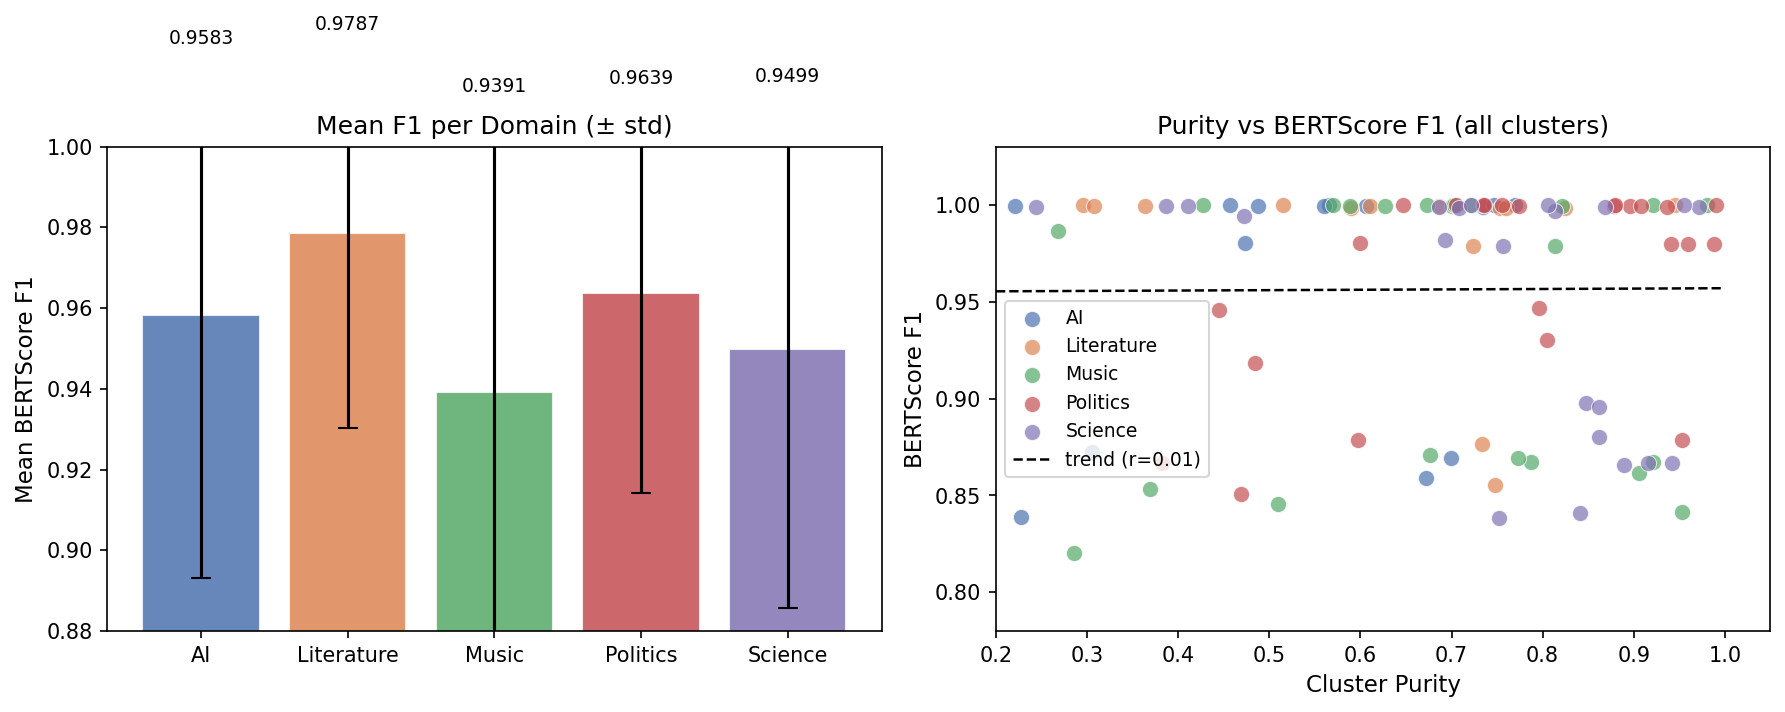
\includegraphics[width=\textwidth]{../figure/naming_summary.png}
      \vspace{0.2em}
      \footnotesize
      \textbf{Left}: mean BERTScore-F1 $\pm$std per domain.\\
      \textbf{Right}: cluster purity vs.\ BERTScore-F1;\\
      \hg{$r = 0.01$} — naming quality is \textbf{independent}\\
      of cluster purity. LLM recovers semantics\\
      even from impure clusters.
    \end{column}
  \end{columns}
\end{frame}

% ------------------------------------------------------------------
% SLIDE 23 — ABLATION STUDY
% ------------------------------------------------------------------
\begin{frame}{Ablation Study: Contribution of Each Component}
  \begin{columns}[T]
    \begin{column}{0.5\textwidth}
      \footnotesize
      \setlength{\tabcolsep}{3pt}
      \renewcommand{\arraystretch}{1.3}
      \begin{tabular}{l|ccccc|c}
        \toprule
        \textbf{Model} & AI & Lit & Mus & Pol & Sci & \textbf{Avg} \\
        \midrule
        OWNER (baseline) & 44.3 & 46.6 & 50.1 & 53.7 & 52.3 & 49.4 \\
        w/o Soft Prompt  & 52.3 & 56.3 & 57.5 & 63.9 & 62.8 & 58.6 \\
        w/o Ensemble MD  & 49.3 & 53.0 & 58.8 & 64.1 & 63.8 & 57.8 \\
        \rowcolor{gold!25}
        \textbf{Full Model} & \textbf{57.6} & \textbf{56.9} & \textbf{60.0} & \textbf{66.3} & \textbf{66.0} & \textbf{61.4} \\
        \bottomrule
      \end{tabular}
      \vspace{0.5em}
      \normalsize
      \textbf{Conclusions:}
      \begin{enumerate}
        \item DTrans multi-view: \hg{$+9.2$} — largest single gain
        \item Soft prompt: \hg{$+2.8$} — on top of DTrans
        \item Both contribute independently: removing either causes a drop
      \end{enumerate}
    \end{column}
    \begin{column}{0.5\textwidth}
      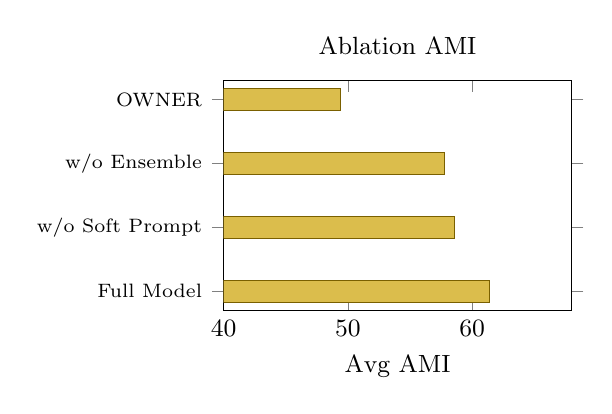
\begin{tikzpicture}
        \begin{axis}[
          xbar,
          width=6cm, height=4.5cm,
          symbolic y coords={Full Model, w/o Soft Prompt, w/o Ensemble, OWNER},
          ytick=data,
          y tick label style={font=\scriptsize},
          xlabel={Avg AMI},
          xmin=40, xmax=68,
          bar width=8pt,
          ymajorgrids=false,
          title={\small Ablation AMI}]
          \addplot[fill=gold!70,draw=gold!60!black] coordinates {
            (61.4,Full Model)
            (58.6,w/o Soft Prompt)
            (57.8,w/o Ensemble)
            (49.4,OWNER)};
        \end{axis}
      \end{tikzpicture}
      \vspace{0.4em}
      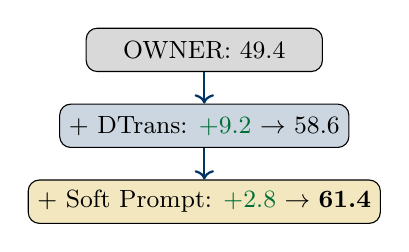
\begin{tikzpicture}[node distance=0.4cm,
          box/.style={draw,rounded corners,minimum width=3cm,
                      minimum height=0.55cm,align=center,font=\small}]
        \node[box,fill=gray!30] (a) {OWNER: 49.4};
        \node[box,fill=navyblue!20,below=of a]
          (b) {+ DTrans: \hg{$+9.2$} $\to$ 58.6};
        \node[box,fill=gold!25,below=of b]
          (c) {+ Soft Prompt: \hg{$+2.8$} $\to$ \textbf{61.4}};
        \draw[->,thick,navyblue] (a)--(b);
        \draw[->,thick,navyblue] (b)--(c);
      \end{tikzpicture}
    \end{column}
  \end{columns}
\end{frame}

% =============================================================
\section{Discussion}
% =============================================================

% ------------------------------------------------------------------
% SLIDE 24 — DISCUSSION
% ------------------------------------------------------------------
\begin{frame}{Discussion: Key Findings \& Insights}
  \begin{columns}[T]
    \begin{column}{0.5\textwidth}
      \textbf{Why CoNLL outperforms Pile-NER?}
      \begin{itemize}
        \item CrossNER is Wikipedia-style formal text
        \item CoNLL-2003 newswire $\approx$ similar syntax and capitalization conventions
        \item Pile-NER: broader vocab but \emph{noisier, colloquial}
        \item \hl{Source-target stylistic alignment $>$ vocabulary breadth}
      \end{itemize}
      \vspace{0.4em}
      \textbf{Cascade effect: detection $\to$ AMI}
      \begin{itemize}
        \item Span F1 gain: $+6.67$
        \item AMI gain: $+12.0$
        \item End-to-end gain \textbf{exceeds} raw detection gain
        \item Hypothesis: better spans $\to$ cleaner [MASK] representations $\to$ more coherent clusters
      \end{itemize}
    \end{column}
    \begin{column}{0.5\textwidth}
      \textbf{When does MMR hurt?}
      \begin{itemize}
        \item Music domain: OWNER random (0.957) $>$ MMR (0.939)
        \item Music clusters are \textbf{tight \& homogeneous}:\\
          \textit{band}, \textit{genre}, \textit{album} — unambiguous
        \item MMR's diversity pressure selects peripheral outliers $\to$ noise
        \item \hl{Rule: use MMR for heterogeneous clusters;\\centroid-nearest for tight clusters}
      \end{itemize}
      \vspace{0.4em}
      \textbf{Naming $\perp$ clustering quality}
      \begin{itemize}
        \item Pearson $r = 0.01$ between cluster purity and BERTScore
        \item LLM can identify dominant type even from impure clusters
        \item Improving $k$ estimation benefits AMI, not naming quality
      \end{itemize}
    \end{column}
  \end{columns}
\end{frame}

% =============================================================
\section{Conclusion}
% =============================================================

% ------------------------------------------------------------------
% SLIDE 25 — CONTRIBUTIONS SUMMARY
% ------------------------------------------------------------------
\begin{frame}{Summary of Contributions}
  \begin{columns}[T]
    \begin{column}{0.6\textwidth}
      \vspace{0.2em}
      \begin{enumerate}
        \setlength{\itemsep}{0.6em}
        \item \textbf{Multi-view entity detection}\\
          DTrans: BIO + SE + TB + Mean Teaching\\
          Span F1: 75.68 $\to$ \hg{82.35} ($+6.67$)\\
          Largest gain in AI domain: $+20.85$

        \item \textbf{Two-stage soft-prompt entity typing}\\
          Only $3{,}840$ trainable parameters\\
          Stage 1: prompt warmup ($3\times10^{-3}$)\\
          Stage 2: full model ($1\times10^{-5}$)\\
          AMI contribution: \hg{$+2.8$ points}

        \item \textbf{MMR-based cluster naming}\\
          $K_e=16$ diverse exemplars, $\lambda=0.7$\\
          LLM backend: 0.956 avg BERTScore-F1\\
          \hg{$+0.012$ over random selection} (budget-controlled)
      \end{enumerate}
    \end{column}
    \begin{column}{0.38\textwidth}
      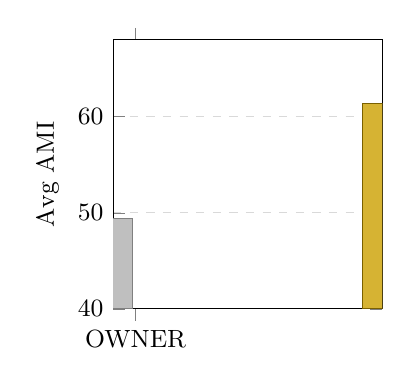
\begin{tikzpicture}
        \begin{axis}[
          ybar, bar width=12pt,
          width=5cm, height=5cm,
          ylabel={Avg AMI},
          symbolic x coords={OWNER,Span2Type},
          xtick=data,
          ymin=40, ymax=68,
          ymajorgrids=true,
          grid style={dashed,gray!30}]
          \addplot[fill=gray!50,draw=gray] coordinates {(OWNER,49.4)};
          \addplot[fill=gold!80,draw=gold!60!black]
            coordinates {(Span2Type,61.4)};
        \end{axis}
      \end{tikzpicture}
      \vspace{0.2em}
      \begin{exampleblock}{\centering End-to-End Result}
        \centering
        \textbf{Span2Type (CoNLL)}\\
        \textbf{61.4} avg AMI\\
        vs.\ OWNER 49.4\\
        \hg{$\Delta = +12.0$ points}
      \end{exampleblock}
    \end{column}
  \end{columns}
\end{frame}

% ------------------------------------------------------------------
% SLIDE 26 — LIMITATIONS & FUTURE WORK
% ------------------------------------------------------------------
\begin{frame}{Limitations \& Future Work}
  \begin{columns}[T]
    \begin{column}{0.5\textwidth}
      \textbf{Current Limitations:}
      \vspace{0.3em}
      \begin{itemize}
        \setlength{\itemsep}{0.4em}
        \item Detector still requires labeled \textbf{source domain}\\
          (newswire $\to$ clinical text: large gap)
        \item \textbf{BIC overestimates $k$} for imbalanced domains\\
          (Politics: 24 predicted vs.\ 9 gold types)
        \item MLM names: limited to single token\\
          LLM names: requires locally hosted model
        \item MMR counterproductive for tight, homogeneous clusters (Music)
      \end{itemize}
    \end{column}
    \begin{column}{0.5\textwidth}
      \textbf{Future Directions:}
      \vspace{0.3em}
      \begin{enumerate}
        \setlength{\itemsep}{0.4em}
        \item \textbf{Domain-adaptive pretraining} or self-training to bridge larger source-target gaps
        \item \textbf{LoRA / adapters} for entity typing — more expressive than $5\times768$ soft tokens
        \item \textbf{Hierarchical clustering} to produce entity type \emph{ontologies} rather than flat partitions
        \item \textbf{MMR at training time} — diverse in-context retrieval during entity typing
        \item Evaluate on \textbf{biomedical \& legal domains} where open-world NER is most needed
      \end{enumerate}
    \end{column}
  \end{columns}
  \vspace{0.4em}
\end{frame}

% ------------------------------------------------------------------
% SLIDE 27 — THANK YOU
% ------------------------------------------------------------------
\begin{frame}[plain]
  \begin{tikzpicture}[remember picture,overlay]
    \fill[navyblue] (current page.north west) rectangle (current page.south east);
    \node[font=\Huge\bfseries,white] at (current page.center)
      {Thank You};
    \node[font=\large,gold,yshift=-1.3cm]
      at (current page.center) {Questions \& Discussion Welcome};
    \node[font=\small,white!80,align=center,yshift=-2.8cm]
      at (current page.center){%
        Nguyen Minh Khoa \quad
        \texttt{18520923@gm.uit.edu.vn} \\[4pt]
        \textit{Span2Type: Open World Named Entity Recognition with Automatic Entity Naming}};
  \end{tikzpicture}
\end{frame}

% =============================================================
%  APPENDIX
% =============================================================
\appendix
\setbeamertemplate{footline}[frame number]

\begin{frame}{Appendix A — Naming Examples (Qualitative)}
  \small
  \begin{tabular}{l|ll|ll}
    \toprule
    Domain & \textbf{GT Type} & \textbf{LLM Name} & \textbf{GT Type} & \textbf{MLM Name} \\
    \midrule
    AI         & researcher   & computer scientist & conference  & conference \\
    Literature & writer       & novelist           & book        & novel \\
    Music      & musicalartist & musician          & band        & band \\
    Politics   & politician   & political leader   & politicalparty & democrat \\
    Science    & protein      & biological protein & scientist   & physicist \\
    \bottomrule
  \end{tabular}
  \vspace{0.5em}

  \textbf{Failure patterns:}
  \begin{itemize}
    \item \textbf{Specificity mismatch}: LLM predicts hyponym (\textit{actor} for \texttt{person})
    \item \textbf{Compound label penalty}: \texttt{musicalartist} vs.\ \textit{musical artist} — semantically correct but tokenization mismatch reduces BERTScore
    \item \textbf{MLM hallucination}: \textit{vegetarian} — BERT defaults to high-frequency unrelated token for OOD context. LLM backend is immune.
  \end{itemize}
\end{frame}

\begin{frame}{Appendix B — Literature Domain Per-Cluster Naming}
  \small
  \begin{tabular}{c|l|l|c|c}
    \toprule
    \textbf{Cluster} & \textbf{GT Type} & \textbf{LLM Name} & \textbf{BERTScore} & \\
    \midrule
    C1  & person       & author           & 0.994 & \cmark \\
    C2  & book         & novel            & 0.998 & \cmark \\
    C3  & location     & theatre          & 0.979 & \hl{$\sim$} \\
    C4  & writer       & poet             & 0.992 & \cmark \\
    C5  & book         & mythology        & 0.996 & \cmark \\
    C6  & literarygenre & literary genre  & 0.993 & \cmark \\
    C7  & award        & literary award   & 0.998 & \cmark \\
    C8  & event        & film festival    & 0.877 & \xmark \\
    C13 & literarygenre & literary work   & 0.855 & \xmark \\
    \bottomrule
  \end{tabular}
  \vspace{0.3em}

  Literature = highest domain mean BERTScore-F1 = \textbf{0.979}\\
  11 of 14 clusters score $\geq 0.99$ (green).\\
  C8 failure: specificity mismatch (\textit{film festival} vs.\ broad \texttt{event}).\\
  C13 failure: compound string \texttt{literarygenre} penalizes correct multi-word name.
\end{frame}

\begin{frame}{Appendix C — Why LLM Baselines Underperform}
  LLM-prompting baselines (UniNER, ChatIE) ask the LLM to identify AND type entities in one pass.\\[0.5em]

  \textbf{Three structural weaknesses vs.\ Span2Type:}
  \vspace{0.4em}
  \begin{enumerate}
    \setlength{\itemsep}{0.5em}
    \item \textbf{No explicit span detector}: zero-shot extraction limits recall; the LLM's span boundary decisions are not trained discriminatively on entity data.

    \item \textbf{Inconsistent type strings}: open-vocabulary output from the LLM produces \textit{``a person working in politics''} and \textit{``politician''} for the same type — clustering these together is impossible and AMI scores drop.

    \item \textbf{Structural mismatch with AMI}: AMI measures agreement between predicted and gold \emph{span partitions}; LLM-extracted spans differ structurally from gold annotation boundaries, creating systematic offset even when semantics are correct.
  \end{enumerate}

  \vspace{0.4em}
  Span2Type separates span detection (discriminative), embedding (template), and clustering (unsupervised) into \textbf{well-defined, optimized stages} — each addressing one specific failure mode.
\end{frame}

\begin{frame}{Appendix D — DTrans Full Hyperparameters}
  \footnotesize
  \begin{tabular}{ll}
    \toprule
    \textbf{Hyperparameter} & \textbf{Value} \\
    \midrule
    Backbone & BERT-base-cased (12L, H=768, A=12) \\
    Learning rate & $1\times10^{-5}$ \\
    Batch size & 32 \\
    Training epochs & 50 \\
    Warmup steps & 500 \\
    EMA decay $\alpha$ & 0.995 \\
    Consistency weight $\lambda_w$ & 100 \\
    Max sequence length & 128 tokens \\
    Confidence threshold $\delta$ & 0.5 (default) \\
    Source corpus & CoNLL-2003 / Pile-NER \\
    Hardware & 2$\times$ GPU \\
    \bottomrule
  \end{tabular}
\end{frame}

\end{document}
